% !TeX program = xelatex
% MathorCup 2026 赛道 A 论文（重构版）
\documentclass{mathorcup-journal}
\usepackage{longtable,booktabs,array,hyperref,listings,xcolor}
\geometry{left=2cm,right=2cm,top=2.6cm,bottom=2.6cm}
\setlength{\columnsep}{0.75cm}
\setlength{\columnseprule}{0pt}
\setlength{\tabcolsep}{2.5pt}
\setmonofont{Consolas}
\newcolumntype{L}[1]{>{\raggedright\arraybackslash}p{#1}}
\fancypagestyle{contest}{\fancyhf{}\renewcommand{\headrulewidth}{0pt}\fancyfoot[C]{\thepage}}
\fancypagestyle{plain}{\fancyhf{}\renewcommand{\headrulewidth}{0pt}\fancyfoot[C]{\thepage}}
\pagestyle{contest}
\setlength{\parindent}{2em}
\setlength{\parskip}{0.25em}
\setlength{\emergencystretch}{3em}
\hypersetup{hidelinks}
\lstset{basicstyle=\ttfamily\tiny,breaklines=true,breakatwhitespace=false,
  breakautoindent=false,breakindent=0pt,columns=fixed,keepspaces=true,
  numbers=left,numberstyle=\tiny,frame=single,
  literate={_}{{\char95\allowbreak}}1}
\captionsetup[table]{position=top}
\renewcommand{\figurename}{图}
\renewcommand{\tablename}{表}

\begin{document}
\twocolumn[{\begin{center}{\zihao{2}\heiti 基于评分端点重建与缺陷约束的啤酒风味预测及风格迁移}\end{center}\vspace{1.0em}
\noindent\textbf{摘\quad 要}\quad
针对啤酒化合物到感官画像的预测、关键因素识别与风格迁移三个问题，本文先重建评分端点，再分别建立预测、解释与决策模型。
\par
附件 4 的感官值是逐人中心化后的连续值，不是 0--6 原始分。本文据公开的 2197 条 0--6 评分（16 名品评员，每款酒 3--14 人）重建了 50 个目标的面板均分与七级分布；对8.xlsx的70个参考字段逐项核查：37个符合对数规则、1个恒等对应，另32个字段含80处差异。附件中显式缺失仅 73 格，另有 18.7\% 的输入单元格为负值，其含义需按字段变换规则判断，二者必须分开处理。
\par
第一问按酒三折五次验证。极端随机树与梯度提升树的等权融合在核心 30 项上的面板均分平均绝对误差为 0.50222 分，明显优于训练均值（0.60450 分），却只比风格中位数基线（0.50969 分）低 0.00747 分，差值的 95\% 重采样区间 $[-0.01914,0.00418]$ 含 0：固定预测比较不足以确认融合模型优于已知风格基线；补充的同参数ET对照中，风格加化学相对仅风格的核心MAE低0.01426分，但相对风格中位数的区间仍跨0。七级分布模型的累计分布平方距离为 0.02178（总体基线 0.02820），面板众数一致率 80.52\%，但非零众数一致率仅 24.33\%，总体一致率主要由 78.03\% 的零等级贡献。保形区间逐属性平均覆盖 90.06\%、宽 1.7342 分，按品评人数分组后 3--4 人组降至 74.00\%。缺失机制实验显示，系统性低值缺失使核心误差增加 0.0273 分，约为随机缺失 20\%（0.0139 分）的两倍，不同缺失机制和缺失比例需要共同解释。
\par
第二问以 $|r|\ge0.7$ 构建 231 节点、109 条边的共表达图。图正则模型在单折平均口径下略差于无图（0.537035 对 0.536911），在聚合预测口径下略好（0.524865 对 0.526148），最终模型取 $\lambda=0$；网络主要用于描述共变结构；150 条 Top-3 候选中 36 条满足“频率 $\ge0.5$、至少 5 折入选、置换贡献为正”的条件，将 80 个异常单元格置缺后 Top-3 保留 97.64\%，仅用一致字段与有单位登记字段的32项交集时降至36.18\%。
\par
第三问对 Tripel、Kriek、Lambic 各生成 40 条谱。受约束局部凸组合把 Tripel 的平均目标风格概率提高到 0.3358（重采样 0.2992），判为目标风格的比例为 0.695（重采样 0.565），但分布距离反而更大（0.1158 对 0.1034），说明“更像目标风格”与“更接近真实分布”不是一回事。迁移在 55 条记录上搜索可行 51 条、独立代理支持 11 条；严格浓度协议下最大 Tripel 份额全为 0，且 55 条记录均找到正余量不可行证书，阻塞主要来自 DMS 与反式-2-壬烯醛；改用阈值超额协议后，参考阈值下30条记录允许正份额，但没有候选通过联合代理复核；2倍阈值敏感性下34条允许正份额，其中9条重复划分记录获得代理支持，并未经过实际制备与盲评。
\par
结果显示：风格基线与复杂模型的误差接近；关键因素应按稳定支持与探索性候选分层解释；阈值约束与代理判断显著影响迁移候选，实际效果需要制备和盲评。

\vspace{0.6em}

\noindent\textbf{关键词}\quad 啤酒风味；感官评分重建；有序分布；化合物共表达网络；风格迁移；缺陷阈值约束
\vspace{1.2em}}]
\thispagestyle{empty}
\clearpage
\onecolumn
\begingroup
\small
\setlength{\parskip}{0em}
\tableofcontents
\endgroup
\thispagestyle{empty}
\twocolumn
\setcounter{page}{1}

\section{问题重述与分析}

啤酒的风味由挥发性化合物、理化条件与酿造工艺共同决定：酯类与高级醇带来果香与醇厚感，酒花萜烯提供草本与柑橘调，硫化物、双乙酰、反式-2-壬烯醛等则构成缺陷。附件给出了 250 款商业啤酒的化合物测量与感官评分，要求完成三项任务：由化合物预测 0--6 分的感官画像；识别各感官维度的关键化合物并论证其稳定性与化学合理性；在给定风格下生成化合物谱，并把 Pils/Lager 迁移为 Tripel 而缺陷不恶化。

\subsection{三项任务要求的证据强度不同}

三项任务共享同一份数据与同一套验证框架，但它们要求的证据强度依次递增。第一问是\textbf{预测}：只要在留出酒样上误差可控、区间可信，结论即可成立。第二问是\textbf{解释}：模型选出的重要化合物必须同时满足统计稳定与化学可解释，而相关系数与回归系数都不构成因果。第三问是\textbf{决策}：生成谱与迁移候选要同时满足风格、感官与缺陷三类约束，模型内可行与真实可酿造之间还隔着制备与品评。

因此本文不为三问套用同一种评价：第一问报告按酒划分的留出误差与区间覆盖，第二问报告重采样频率与置换贡献，第三问报告冻结候选的三层复核与线性规划可行性证书。任何一问的好成绩都不自动支持另一问。

\subsection{技术路线}

图\ref{fig:roadmap}给出全文结构。数据层完成四件事：附件结构核查、化学尺度与缺失诊断、评分端点重建、评分卡到目标列的维度映射。任务层按三问展开，但共用同一批按酒分层的划分与同一套预处理规则。最底层是统一的验证约定：插补、截尾、标准化与调参只在训练折内估计，生成与迁移的候选先冻结再复核，失败与反直觉结果全部保留。

\begin{figure*}[t]
\centering
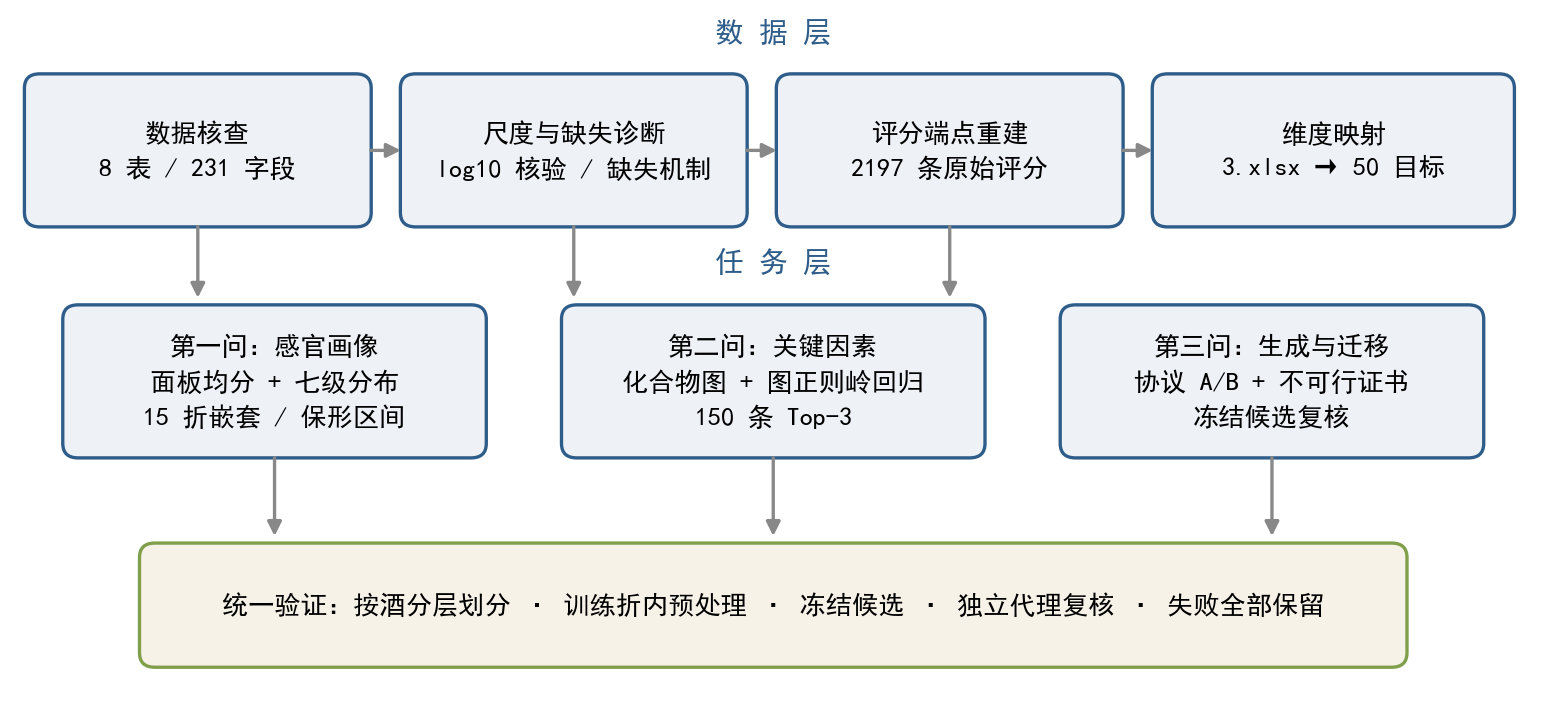
\includegraphics[width=0.98\textwidth]{figures/fig01_roadmap.png}
\caption{全文技术路线。数据层的四项核查共同决定任务层的输入口径；三问共用按酒分层划分与训练折内预处理，避免同一款酒同时出现在训练与验证中。}
\label{fig:roadmap}
\end{figure*}

\subsection{本文的交付物}

对应三问，本文给出四类可复核的结果：一是 250 款酒在 50 个感官目标上的面板均分与七级评分分布，以及据此得到的众数与中位数等级；二是 50 个目标各 3 个候选化合物、共 150 条因素记录，附重采样入选频率、置换贡献与化学依据；三是 Tripel、Kriek、Lambic 三种风格的生成谱及其感官画像；四是 Pils/Lager 到 Tripel 的迁移可行域，包括严格协议下的不可行证书与阈值协议下的可行记录数。

上述结果全部由可重跑的脚本产生，输入文件哈希、随机种子与运行配置随结果保存。第\ref{sec:data}节交代数据口径，第\ref{sec:q1}至\ref{sec:q3}节分别给出三问的模型与结果，第\ref{sec:eval}节讨论适用范围与推广。

\section{模型假设与符号说明}

\subsection{基本假设}

\begin{enumerate}
\item[\textbf{A1}] 附件 1 的字段可能采用对数、恒等或其他处理；对经过核查的对数字段，负值可表示原始浓度小于 1。第\ref{sec:scale}节逐字段比较70个参考字段，不对所有列统一反变换。
\item[\textbf{A2}] 显式缺失（1.csv 中 73 个空单元格）为随机缺失，与化合物浓度无关；低值密集（数值小于 0 的 10797 个单元格）属于检出限以下的观测，不按缺失处理。第\ref{sec:missing}节用四种缺失机制检验该假设的后果。
\item[\textbf{A3}] 附件 4 的连续值是同一批原始评分经逐人中心化、标准化后的结果，可由公开的 2197 条 0--6 原始评分重建出面板均分与七级分布；同一品评员的重复评分可先平均，品评员之间等权。
\item[\textbf{A4}] 风格标签 \texttt{tasting\_category\_fine} 可靠，且风格差异是感官差异的主要来源；因此风格中位数是一个必须比较的强基线，而不是可忽略的对照。
\item[\textbf{A5}] 缺陷阈值取自文献与 8.xlsx 的阈值中位数，可近似迁移到本数据；但阈值依赖啤酒基质与测量方法，故在第三问中把阈值写成可缩放参数，并在 0.5、1、2 倍三档上报告结论。
\item[\textbf{A6}] 面板均分可代表该款酒的感官强度，众数可代表最常见的等级；两者对应不同的决策损失，不能互相替代。
\end{enumerate}

\subsection{符号说明}

表\ref{tab:symbol}汇总全文记号。矩阵用大写粗体，向量用小写粗体，标量用斜体；下标 $b$ 表示酒款、$j$ 表示感官目标、$t$ 表示品评员、$r$ 表示同一品评员的重复次数、$d$ 表示缺陷化合物。

\begin{table}[t]
\centering\small\renewcommand{\arraystretch}{1.15}
\caption{主要符号}
\label{tab:symbol}
\begin{tabular}{L{0.20\columnwidth}L{0.68\columnwidth}}
\toprule
符号 & 含义 \\
\midrule
$n,p,q$ & 酒款数（250）、化合物字段数（231）、感官目标数（50） \\
$X\in\mathbb{R}^{n\times p}$ & 化合物与理化特征矩阵 \\
$Y\in\mathbb{R}^{n\times q}$ & 感官目标矩阵（面板均分） \\
$s_{btrj}$ & 品评员 $t$ 对酒 $b$、目标 $j$ 的第 $r$ 次原始评分 \\
$\bar s_{bj}$ & 酒 $b$ 在目标 $j$ 上的面板均分 \\
$q_{bjk}$ & 酒 $b$ 在目标 $j$ 上取等级 $k$ 的面板比例 \\
$\hat g_{\text{mode}},\hat g_{\text{med}}$ & 预测众数等级、预测中位数等级 \\
$D$ & 累计分布平方距离 \\
$\mathrm{RPS}$ & 有序概率评分 \\
$Z$ & 训练折内标准化后的特征矩阵 \\
$W,L$ & 化合物相关图的带符号权重矩阵、图拉普拉斯矩阵 \\
$B$ & 多目标回归系数矩阵 \\
$\alpha,\lambda$ & 岭惩罚系数、图正则系数 \\
$c_d,t_d,R_d$ & 缺陷 $d$ 的浓度、参考阈值、阈值超额风险 \\
$\boldsymbol{w}$ & 混配中锚点酒的份额向量 \\
$\boldsymbol{M}$ & 混配约束矩阵（各锚点与来源在缺陷上的浓度差） \\
\bottomrule
\end{tabular}
\end{table}

\section{数据核查与评分端点}\label{sec:data}

\subsection{数据全景与样本对应}

八个附件表可按“化学输入—感官目标—评分卡—旁证”四层归并，样本主键在 1.csv、4.csv、7.csv 与 8.xlsx 之间一致。表\ref{tab:data} 汇总了各表的规模、内容与用途：1.csv 是化学主表，4.csv 是感官监督表，2.csv、5.csv、6.csv 给出相关结构，3.xlsx 定义评分维度，7.csv 与 8.xlsx 分别提供评论旁证和外部校准。附件与公开逐人评分的数据来源见\cite{schreurs2024,zenodo2026}。

\begin{table*}[t]
\centering\small\renewcommand{\arraystretch}{1.15}
\caption{八个附件表的规模、内容与本文用途}
\label{tab:data}
\begin{tabular}{@{}>{\raggedright\arraybackslash}p{0.075\textwidth}>{\raggedright\arraybackslash}p{0.135\textwidth}>{\raggedright\arraybackslash}p{0.435\textwidth}>{\raggedright\arraybackslash}p{0.275\textwidth}@{}}
\toprule
文件 & 规模 & 内容 & 本文用途 \\
\midrule
1.csv & $250\times234$ & 3 列样本信息（beer、beer\_id、风格）+ 231 个数值字段：226 个化合物、5 个综合量 & 化学输入；风格标签与样本对齐 \\
2.csv & $231\times231$ & 231 个化学字段的秩相关矩阵（含行名列共 232 列） & 核对相关结构；构建化学网络 \\
3.xlsx & 12 卡 + 汇总 & 12 张 beer\_* 评分卡 + 1 个 summary；单卡 $100\times33$，summary $13\times52$ & 评分维度定义与目标映射 \\
4.csv & $250\times53$ & 3 列样本信息 + 50 个标准化感官目标（15 A + 15 F + 20 其他） & 目标定义与样本对应；不作 0--6 标签 \\
5.csv & $50\times51$ & 50 个感官目标间的 Spearman 矩阵 & 目标相关性核查与分组 \\
6.csv & $44\times51$ & 44 个化学字段 $\times$ 50 个感官目标的 Spearman 矩阵 & 关键因素筛选的旁证；不作因果解释 \\
7.csv & $250\times189$ & 3 列样本信息 + 186 个 Ratebeer 评论感官词 & 旁证；750 个缺失，不作训练标签 \\
8.xlsx & 7 个 sheet & 70 个校准化学字段（$250\times73$）；阈值 261 行（43 个有数值）；SHAP 500 行；MDI 232 行；价格表 & 尺度反查、第三问阈值、重要性交叉核对 \\
\bottomrule
\end{tabular}
\end{table*}

样本规模为 250 款酒、22 种风格。1.csv 的 231 个数值字段由 226 个化合物和 5 个综合量（\texttt{kcalperc}、\texttt{esters\_sum}、\texttt{aroma\_hops\_sum}、\texttt{acids\_sum}、\texttt{sulfur\_sum}）组成；4.csv 的 50 个目标由 15 个 Aroma、15 个 Flavour 和 20 个其他维度组成。1.csv 与 4.csv 均以 beer 为唯一键、beer\_id 为条码辅助键，250 行的风格标签在两表中一致，样本对应可按编号与行序双重核对，风格分层因此可直接复用，不需要另行匹配。风格样本量从 Faro 的 3 款到 Blond 的 31 款，9 种风格不足 10 款，后续按风格分层划分，避免稀有风格整体落入某一折。

\begin{figure}[t]
\centering
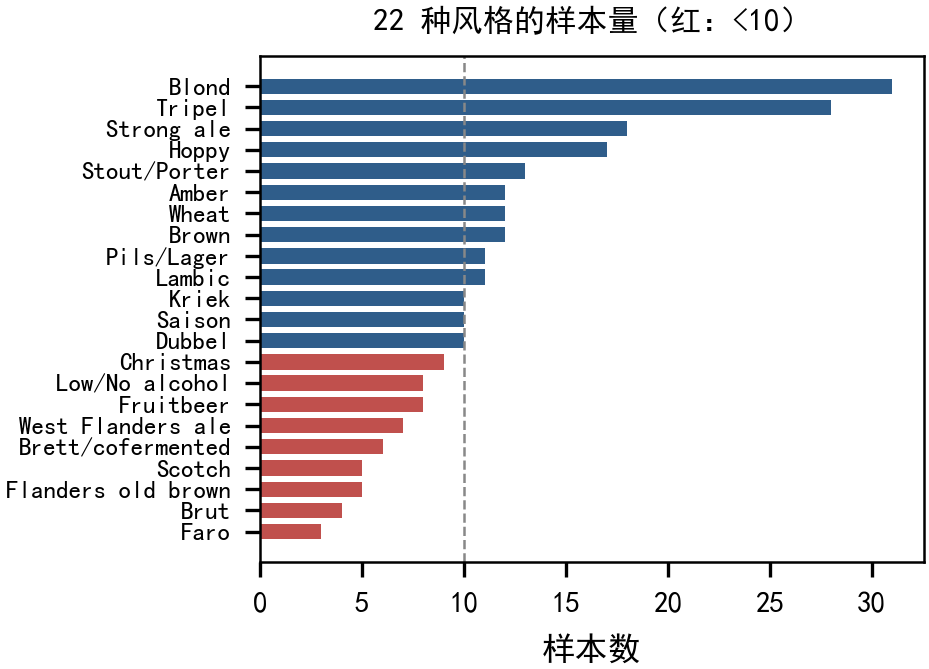
\includegraphics[width=0.95\columnwidth]{figures/fig04_styles.png}
\caption{22 种风格的样本量。红色为不足 10 款的 9 种风格，最少 3 款；分层划分与风格基线都受这一分布约束。}
\label{fig:styles}
\end{figure}5.csv 与 6.csv 分别刻画感官目标之间、化学字段与感官目标之间的秩相关结构；两表用于检查目标分块和因素筛选的方向一致性，不进入预测模型，也不进入第一问特征矩阵，避免把目标间相关当作输入信息造成泄漏。

题面与附件存在三处口径差异，本文以附件为准。题面称 226 款酒，附件为 250 款；题面称约 40 维感官目标，附件为 50 维，其中 Aroma/Flavour 各 15 项、合计 30 项；题面的约 40 维来自两栏各约 20 项的口径，附件把三组汇总和共用维度拆开后为 50 项。题面称评分卡 10 个 sheet，附件为 12 个 beer\_* 评分卡，另加 1 个 summary。四个表共用 beer 编号，使按酒划分训练折时不会出现样本错位。提交口径相应定为：50 项全部建模并输出，30 个核心项单列误差与分布指标，20 个其他项用于缺陷约束和总体评价，不与核心项合并平均。

附件 2 是秩相关矩阵，不是题面所称的皮尔逊相关矩阵。在 212 个可匹配字段上，2.csv 与本地重算 Spearman 的平均绝对差为 $1.6\times10^{-16}$，与 Pearson 的平均绝对差为 0.0883；前者处于机器精度，后者高出一个量级。因此第二问的化学网络按秩相关构建，2.csv 直接作为相关结构使用，题面的“皮尔逊”表述予以纠正。231 个字段中有 19 个因命名或汇总口径无法与 8.xlsx 的化学名匹配，核对只在 212 个可匹配字段上进行；这一限制不影响秩相关判断。8.xlsx 的 7 个 sheet 分别承载校准化学值、感官阈值、SHAP、MDI 与价格；阈值表 261 行中只有 43 行有数值，第三问的缺陷阈值只取有数值的行。

\subsection{化学尺度与异常}\label{sec:scale}

1.csv 包含经不同规则处理的化学与理化字段，不能把所有字段统一按 $10^x$ 还原。以附件 8 校准表与附件 1 中 70 个同名数值字段进行逐字段比较：对每个字段分别测试恒等、非正值替换及替换后取 $\log_{10}$ 的候选规则。38 个字段在全部可比记录上满足数值容差，其中 37 个符合“非正值替换为该字段最小正值的一半，再取 $\log_{10}$”的规则，另一个 \texttt{diethyl.succinate} 满足恒等对应；其余 32 个字段共保留 80 个不一致单元格。两组的 38 和 32 互不重叠，覆盖全部 70 个字段。

对 \texttt{diethyl.succinate}，247 个共同可比记录中，两表原值的最大绝对差为 $5.0\times10^{-10}$。该字段属于恒等对应：若把附件 1 的值误作对数并计算 $10^x/\mathrm{cal}$，比值中位数为 13.95，但各记录范围为 6.26--738.07，说明这是套用不匹配变换产生的差异，不能据此声称该字段有固定倍数的单位偏差。表间一致也不能替代独立仪器标定。

图\ref{fig:scale}(a) 展示 37 个对数规则字段的 8452 个正参考值配对；绘图仅对每个字段使用其原报告单位比较，零值替换记录不在该图中。(b) 按字段统计 80 处例外，排名前八的字段分别列出，其余24字段合并。两幅子图使用不同的数量口径，完整字段分类、变换规则和异常数见附录\ref{app:fieldsets}与支撑材料。

\begin{figure*}[t]
\centering
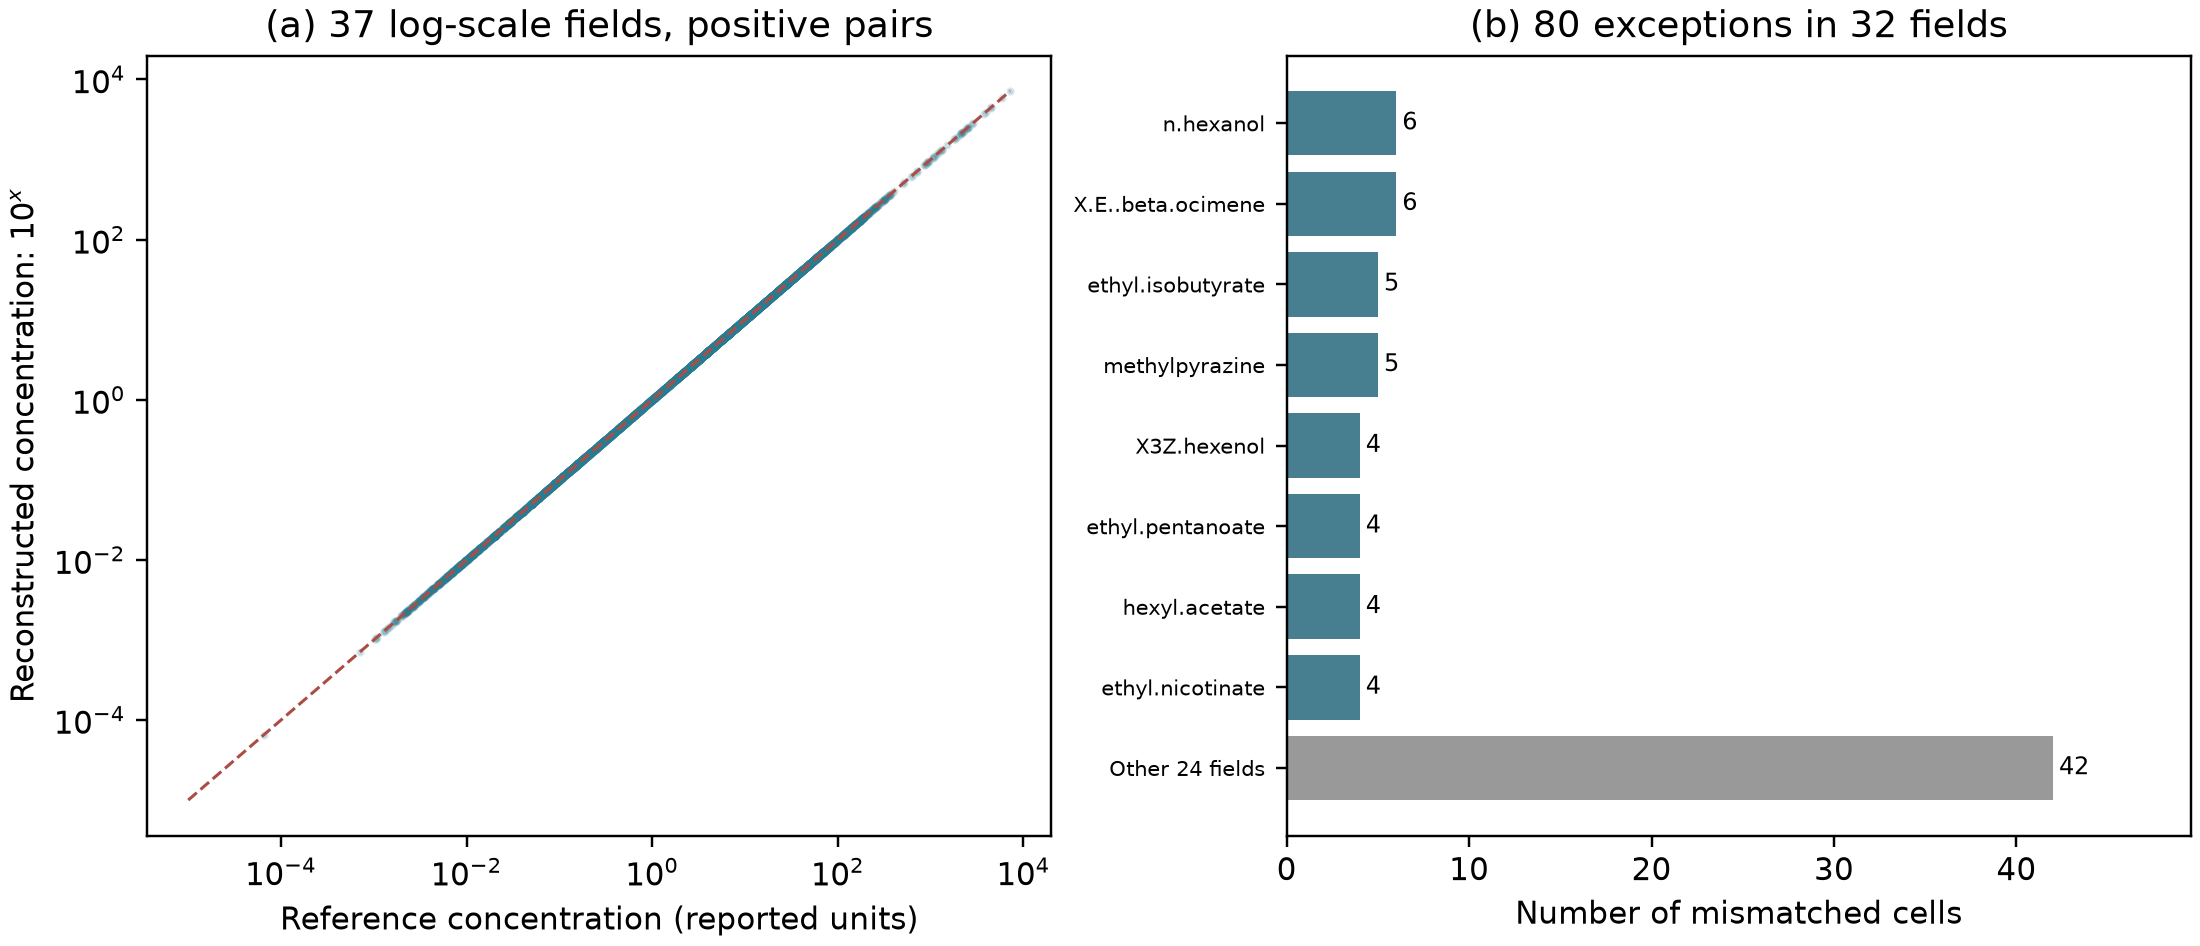
\includegraphics[width=0.98\textwidth]{figures/fig02_scale.png}
\caption{化学尺度核查。(a) 37 个对数规则字段的正值配对，各字段按自身报告单位比较；(b) 32 个不一致字段中异常单元格的数量分布，前八字段单列，其余24字段合计。}
\label{fig:scale}
\end{figure*}

第二问的另一组 32 个字段记为 $V=R\cap U\cap X_{226}$：$R$ 是上述 38 个全部可比记录一致字段，$U$ 是单位注册表中的61个字段，$X_{226}$ 是剔除5个综合量后的非综合输入。$V$ 包括31个对数规则字段和1个恒等对应字段，与80处例外所涉及的32个字段交集为空。该交集仅说明数值对应和单位记录具备，不构成完整化学标定；具体字段与单位列在附录\ref{app:fieldsets}。异常处理敏感性保留原始字段并将80处单元格置缺，填补参数只由训练折估计；另一项对照则更换为 $V$，两者回答不同问题。

\begin{table}[t]
\centering\small
\caption{化学尺度核查的集合定义}
\label{tab:scale}
\begin{tabular}{@{}p{.45\columnwidth}p{.16\columnwidth}p{.30\columnwidth}@{}}
\toprule
集合 & 字段数 & 核查结果\\
\midrule
逐点一致 $R$ & 38 & 37 对数规则、1 恒等规则\\
有例外字段 $E$ & 32 & 共80个异常单元格\\
敏感性子集 $V$ & 32 & $R\cap U\cap X_{226}$；$V\cap E=\varnothing$\\
\bottomrule
\end{tabular}
\end{table}

\subsection{缺失、低值和变换}\label{sec:missing}

显式缺失只有 73 格（0.126\%），但低值密集覆盖 18.7\% 的数值单元格，两者性质不同。73 个缺失分布在 9 列、63 款酒上，最多的一列是 \texttt{amyl.acetate} 的 27 格；9 列中 4 列的缺失不超过 2 格，\texttt{amyl.acetate} 一列接近全部缺失的 37\%。缺失列中既有建模需要的香气化合物，也有 1 个综合量 \texttt{aroma\_hops\_sum}；整列删除会改变输入维度，综合量又不能按单列均值填补，否则会破坏它与子项的关系，故按单元格保留。缺失呈点状分布，没有整行删除；本文不删除缺失行，树模型与线性模型均使用训练折估计的中位数进行填补，避免测试折信息泄漏。

数值小于 0 的单元格有 10797 个，占 18.7\%，175 个字段出现过负值。1.csv 存的是 $\log_{10}$ 浓度，负值对应原始浓度小于 1，属于低值密集而不是缺失；若按缺失删除，会丢掉近两成有效信息并系统性剔除低浓度样本。低值密集不是数据质量问题，而是浓度量级分布的直接结果，负值携带的是低浓度信息；负值占比在不同化合物间差异很大，说明低值密集不是全局缩放造成的，而是各化合物的浓度分布不同。本文保留负值，树模型直接使用，线性模型只在训练折内估计标准化参数。

7.csv 的 750 个缺失集中在 3 列，且 186 个字段来自 Ratebeer 评论词，不是品评小组的 0--6 评分。750 个缺失对应 3 个整列缺失，说明这些感官词在评论语料中没有覆盖，而不是随机漏填；评论词的出现还受文本长度和用户习惯影响，缺失机制不是随机的。因此 7.csv 只作旁证，不能作训练标签；它的 186 个评论词与 4.csv 的 50 个目标并非同一套词表，不能按名称直接合并，若用评论词训练，会把文本噪声当成感官信号。

\begin{figure*}[t]
\centering
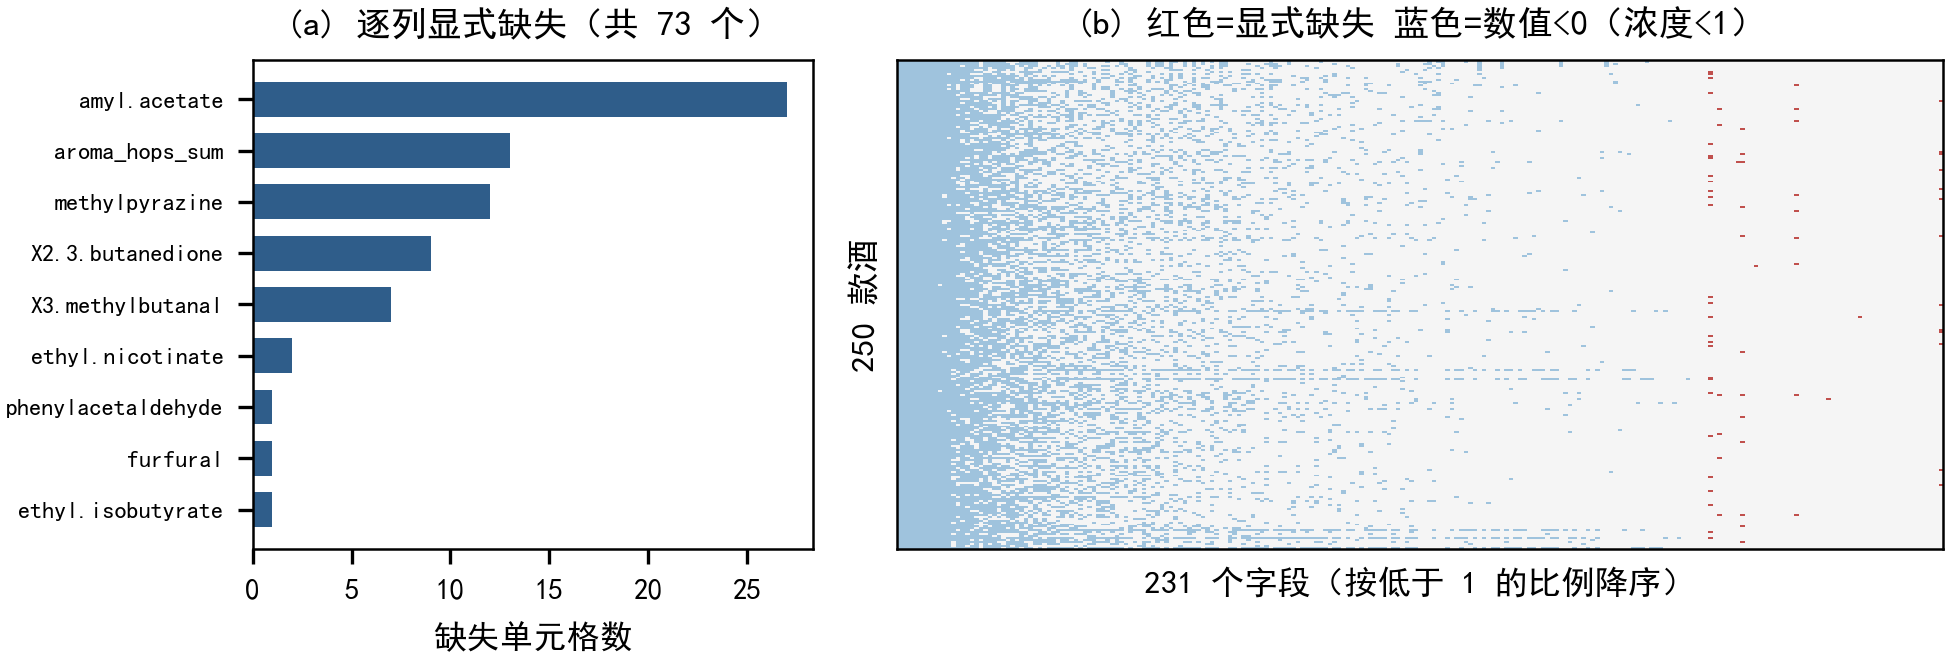
\includegraphics[width=0.98\textwidth]{figures/fig03_missing.png}
\caption{缺失与低值结构。(a) 231 个数值字段的显式缺失量，9 列有缺失，\texttt{amyl.acetate} 最多 27 格；(b) $250\times231$ 矩阵中缺失与负值的空间分布，缺失呈点状，负值呈面状。}
\label{fig:missing}
\end{figure*}

图\ref{fig:missing}(a) 显示显式缺失的列分布，(b) 显示 $250\times231$ 矩阵中缺失与负值的空间分布：缺失是点状，负值是面状。真正影响建模的是低值密集和评分端点的覆盖不足，而不是 73 个显式缺失；4.csv 没有 NaN，但每款酒只有 3--14 名品评员，端点估计的不确定性随人数下降。显式缺失由训练折填补处理，低值密集需要在对数尺度上建模，评分端点的覆盖不足只能通过面板聚合和区间估计控制。

\subsection{评分端点重建}

4.csv 是标准化后的感官分值，不能直接当作 0--6 分标签；0--6 端点需由公开逐人评分重建。4.csv 为 $250\times53$，50 个目标列的均值为 $-0.063$～$0.063$、标准差为 0.37～0.86，符合中心化/标准化后的尺度，与 0--6 原始分不符。各列均值接近 0、标准差小于 1，说明 4.csv 是对原始 0--6 分做中心化/标准化后的结果；列间标准差不齐，说明标准化未统一到单位方差。该表用于样本对应、目标定义和标准化核查，不作为回归标签；它仍保留样本间的相对差异，可用于检查目标分布和异常酒样，但不能还原 0--6 分，也不能替代逐人评分。面板均分的取值范围仍是 0--6，而 4.csv 的标准化值可正可负，两者不能在同一损失函数下混用；4.csv 的列均值和标准差只能确认标准化，不能反推出原始 0--6 分的线性变换参数。

8.xlsx 的字段说明指向作者公开的逐人评分数据。据此重建的面板包含 16 名品评员，每款酒 3--14 人、中位 8 人，共 2197 条 0--6 评分。16 名品评员以匿名编号出现，每款酒的品评员集合不同；按 beer 编号与附件对齐后，30 个 Aroma/Flavour 属性分成两组核对，20 个共用项单独核对。面板人数不等意味着端点精度不等，直接比较不同酒的均分会把精度差异混入误差。2197 条评分是重建端点的全部原始信息；任何汇总都会损失一部分分布信息，故本文保留逐条评分用于分布端点。

记第 $b$ 款酒、第 $j$ 个属性、第 $t$ 名品评员的第 $r$ 次评分为 $s_{btrj}$，$T_b$ 为评过该酒的品评员集合，$n_{bt}$ 为同一人的重复次数。面板均分为
\begin{equation}\label{eq:panelmean}
\bar s_{bj}=\frac{1}{|T_b|}\sum_{t\in T_b}\frac{1}{n_{bt}}\sum_{r=1}^{n_{bt}}s_{btrj},
\end{equation}
七级分布为
\begin{equation}\label{eq:dist}
q_{bjk}=\frac{1}{|T_b|}\sum_{t\in T_b}\frac{1}{n_{bt}}\sum_{r=1}^{n_{bt}}\mathbf{1}\{s_{btrj}=k\},
\end{equation}
其中 $k=0,\ldots,6$。

分母 $|T_b|$ 是实际评过该酒的品评员数，不是全体 16 人；每款酒的端点只使用自己的面板，未评人员不按 0 分计入。式\eqref{eq:panelmean} 与式\eqref{eq:dist} 都先在人内对重复评分取平均，再在人之间等权平均。同一人对同一杯酒的重复评分高度相关，若按原始条目数加权，评分次数多的人会主导端点；等权处理则让每名品评员对一款酒只投一票。同一人可能对同一杯酒给出多次评分，$n_{bt}$ 可能大于 1；先平均再等权等价于把每人的重复评分压缩成一条观测。面板均分与七级分布共享同一套人员权重，因此二者的差异只来自汇总方式，不来自样本集合。

平方损失下均值最优，绝对损失下中位数最优，累计分布损失下完整分布最优，0--1 损失下众数最优。三种端点对应三种决策损失：面板均分对应平方损失，七级分布对应累计分布或 RPS 损失，众数 $\hat g_{bj}=\arg\max_k q_{bjk}$ 对应 0--1 精确等级损失。本文不把三者压成一个标签，而是在第一问分别报告均分误差、分布距离和众数一致率。3--4 人面板的端点不确定性明显大于 8 人以上面板，第一问按人数分组报告覆盖率和误差，避免把面板人数差异误判为模型差异；众数对人数少的面板更敏感，3--4 人时众数可能只反映一两个品评员的选择。

\subsection{维度映射与提交口径}

评分卡与 4.csv 的目标可按字典一一映射，但字段名和模板公式不能直接照搬。3.xlsx 含 12 个 beer\_* 评分卡和 1 个 summary，12 张评分卡对应 12 款示例酒，summary 汇总这些酒的目标列；评分卡只用于维度定义，不直接提供 250 款酒的得分。每张卡左栏 Aroma、右栏 Flavour，两栏各含 Malt、Hops、Esters 三组，每组 4 个描述词加 1 个组汇总；乙醛 1 项，口感 4 项，缺陷 6--7 项，另有香料与 Lambic 专项。映射结果见表\ref{tab:dims}：A/F 前缀各 15 项，共 30 项核心；其余 20 项为口感、缺陷、香料、酸味与总体。这 50 个目标列同时定义第一问的输出、第二问的响应变量和第三问的感官画像维度。

\begin{table*}[t]
\centering\small\renewcommand{\arraystretch}{1.15}
\caption{评分卡分组与 4.csv 目标的字典映射。A/F 前缀各 15 项，其余 20 项为共用目标；乙醛项没有独立目标列。}
\label{tab:dims}
\begin{tabular}{@{}>{\raggedright\arraybackslash}p{0.155\textwidth}>{\raggedright\arraybackslash}p{0.555\textwidth}>{\raggedright\arraybackslash}p{0.105\textwidth}>{\raggedright\arraybackslash}p{0.075\textwidth}@{}}
\toprule
评分卡分组（项数） & 4.csv 字段 & 归属 & 目标数 \\
\midrule
Malt（4 子项 + 1 汇总） & A\_malt\_all, A\_malt\_grain, A\_malt\_bread, A\_malt\_cara, A\_malt\_burn；F 侧同构 & A\_/F\_ & 10 \\
Hops（4 子项 + 1 汇总） & A\_hops\_all, A\_hops\_citrus, A\_hops\_tropical, A\_hops\_noble, A\_hops\_woody；F 侧同构 & A\_/F\_ & 10 \\
Esters（4 子项 + 1 汇总） & A\_esters\_all, A\_esters\_ethac, A\_esters\_isoaa, A\_esters\_flower, A\_esters\_fruity；F 侧同构 & A\_/F\_ & 10 \\
Acetaldehyde（1） & — & — & 0 \\
口感（4） & body, bitternes, co2, aftertaste & 共用 & 4 \\
缺陷（6--7） & dms, metallic, X4vg, diacetyl, t2n, stale\_hops, barnyard & 共用 & 7 \\
香料、酸味与总体（9） & acidity, sweetness, orange, coriander, clove, lactic, acetic, alcohol, overall & 共用 & 9 \\
\midrule
合计 & A 15 项、F 15 项、共用 20 项 & & 50 \\
\bottomrule
\end{tabular}
\end{table*}

4.csv 中 A\_malt\_*、A\_hops\_*、A\_esters\_* 各 5 项，F 侧同构；组汇总以 \_all 结尾，共 6 项，三组汇总分别为 A/F\_malt\_all、A/F\_hops\_all、A/F\_esters\_all，组汇总与 4 个描述词共同构成 5 项，不能只取子项而漏掉汇总。Aroma 栏可映射 15 项（3 组 $\times$ 5），Flavour 栏同理；口感 4 项、缺陷 7 项、香料与总体 9 项构成其余 20 项。乙醛 1 项在 4.csv 中没有独立目标列，故不进入 50 项目标。字段名差异来自评分卡模板与监督表的两次命名：A/F\_ester\_fruity 在 4.csv 中写作 A/F\_esters\_fruity，4vg 写作 X4vg；若按字符串直接匹配，这几个字段会丢失。本文按显式字典映射，字典以 4.csv 的 50 个列名为准，逐项记录评分卡组别、A/F 归属和是否汇总；映射表写入交付包的字段清单，预测时按列名而非列序取数，不依赖评分卡模板公式。bitternes 等拼写按原表保留，避免合并时产生重复列。

提交口径为 50 项全部建模并输出，核心 30 项单列；20 个其他项用于缺陷约束、风格画像和总体评价。核心 30 项是训练面板的主评分维度，20 个其他项多为缺陷或风格专项，两类项目的量纲和稀疏性不同，分开报告更便于按决策场景取用。评分卡的组别划分与 0--6 强度标度符合训练面板的感官评价流程\cite{schreurs2024}；但乙醛位置没有独立目标列，组汇总也不能按模板公式直接重算，直接套公式会把无监督项算进目标，因此本文以字段名和组别字典为准。预测输出按 50 列对齐 4.csv 的列序，核心 30 项与其余 20 项用同一套字段清单标记，便于下游按组取用；映射表同时作为训练、预测和评价三处的字段白名单，避免不同脚本各自解释列名。

\section{第一问：感官画像的预测}\label{sec:q1}

第一问要求仅凭 231 个数值输入（226 个化合物与 5 个综合量）预测 50 项感官画像。本文把画像拆成均值、分布和等级三层输出，三层各有对应的损失与评价口径；均分与分布的模型比较在同一套按酒划分的 15 个留出折上完成，区间与缺失实验另设划分，后文分别注明。

\subsection{三类输出与评价指标}

第一问的交付物是三类可分别评价的输出，而不是一个等级。第 3 节已把第 $b$ 款酒、第 $j$ 个属性的面板均分记为 $\bar s_{bj}$，把七级评分分布记为 $q_{bjk}$；本节沿用这两组记号。

交付物包括连续的面板均分 $\bar s_{bj}\in[0,6]$、七维概率 $(q_{bj0},\ldots,q_{bj6})$（非负且和为 1），以及由分布导出的众数等级与中位数等级；前两者描述平均强度与评分分歧，后者给出整数决策。众数取概率最大的等级，中位数取累计概率首次达到 0.5 的等级；在零膨胀的偏态分布下两者经常不同，不能互相替代。

三类输出对应三种决策。若只需要一个总体强度，取面板均分；若要报告不确定性，取七级分布；若必须给出一个整数等级，才在众数和中位数之间选择。把三者压成一个数字，会丢失评分分歧，也会让评价口径随下游任务漂移。

面板均分用平均绝对误差评价：

\begin{equation}
\mathrm{MAE}=\frac{1}{nm}\sum_{b=1}^{n}\sum_{j=1}^{m}\left|\bar s_{bj}-\hat s_{bj}\right|.
\label{eq:mae}
\end{equation}

其中 $n$ 为酒数，$m$ 为核心 30 项或全 50 项，$\hat s_{bj}$ 为留出预测。MAE 的单位是分，可直接与 0—6 的评分尺度对照。

分布质量用累计分布平方距离评价。记某款酒某属性的预测概率为 $\hat p_h$、观测分布为 $q_h$，$P_k=\sum_{h=0}^{k}\hat p_h$ 与 $Q_k=\sum_{h=0}^{k}q_h$ 分别为预测分布与观测面板分布在等级边界 $k$ 的累计概率，则

\begin{equation}
D=\frac{1}{6}\sum_{k=0}^{5}\left(P_k-Q_k\right)^2.
\label{eq:cdd}
\end{equation}

式\eqref{eq:cdd} 对六个内部边界取平均，使 $D$ 与七级概率处于同一尺度；逐条记录计算后取平均，得到表\ref{tab:ordinal} 中的 $D$。$D$ 越小，预测分布越接近该酒实际的面板经验分布。

若把预测分布发给一位随机抽出的品评员，其实际等级为 $Y$，则单次评分的秩序概率评分为

\begin{equation}
\mathrm{RPS}(P,Y)=\frac{1}{6}\sum_{k=0}^{5}\left(P_k-\mathbf{1}\{Y\le k\}\right)^2.
\label{eq:rps}
\end{equation}

式\eqref{eq:rps} 是严格适当的评分规则，鼓励模型报告真实概率而不是把质量压向某一等级\cite{gneiting2007}。对 $Y\sim q$ 取期望，并记面板分歧项 $\Delta=\frac{1}{6}\sum_{k=0}^{5}Q_k(1-Q_k)$，则

\begin{equation}
\mathbb{E}_{Y\sim q}\left[\mathrm{RPS}(P,Y)\right]=D+\Delta.
\label{eq:rpsdecomp}
\end{equation}

式\eqref{eq:rpsdecomp} 说明个人期望 RPS 由两部分组成：第一部分正是 $D$，第二部分 $\Delta$ 只由观测分布的分歧程度决定。核心 30 项上 $D=0.02178$、期望 RPS $=0.11044$，两者相差 $0.08866$，恰好等于面板分歧项的平均值。把 $0.02178$ 称为 RPS，或把 $0.11044$ 当作分布距离，都会把“分布拟合”和“个人评分预测”混为一谈；本文对两者分别报告、分别解释。

从数值看，分歧项 0.08866 远大于 $D$ 的 0.02178，其中分歧项来自面板经验评分分布的离散度；它反映人员及重复评分差异，不能单独识别其成因。这决定了后文的改进重点：继续压低 $D$ 的空间有限，提高个人等级命中率更困难。

\subsection{面板均分预测}

风格中位数是较强的已知风格基线；融合模型与其误差差距较小，需要结合不确定性解释。

面板均分预测以 15 个留出折评价：按风格分层、以酒为单位做三折，重复五次，每款酒在五次中各被留出一次；先把五次留出预测取平均，再按式\eqref{eq:mae} 计算 MAE。这样同一款酒只贡献一个误差，避免重复留出被当作独立样本。

比较的方法包括训练均值、总体中位数、风格中位数、岭回归、极端随机树、梯度提升树，以及极端随机树与梯度提升树的固定等权融合\cite{geurts2006,friedman2001,breiman1996,wolpert1992}。岭回归的正则系数在训练折内选择，其余方法使用预先固定的参数。

三折而非五折，是因为 22 种风格中有 9 种少于 10 款、最少只有 3 款；三折能保证每个训练折仍覆盖全部风格，五次重复则降低单次划分的偶然性。融合权重固定为等权而不是在留出折内学习，是为了避免把模型选择误差带进比较；风格中位数对每个目标只估计一组风格常数，参数个数等于风格数，因而是一个很强的朴素基线。

结果见表\ref{tab:mae}。融合在核心 30 项上的 MAE 为 0.50222 分，在全部 50 项上为 0.43560 分；相对训练均值的降幅分别为 0.10228 分和 0.11319 分。真正需要解释的是这 0.10228 分从哪里来。风格中位数只使用风格标签、不使用任何化合物，核心 MAE 已达 0.50969 分；使用 231 个化学输入的融合模型只把误差压到 0.50222 分，融合低 0.00747 分。

以酒为单位、在固定预测条件下重采样，融合减风格中位数的差值 95\% 区间为 $[-0.01914,0.00418]$，含 0。在本数据与固定预测的重采样口径下，没有足够证据确认融合模型优于风格中位数；这不等于证明化合物信息的条件增量为零。风格中位数到总体均值的误差差，占总体均值到融合模型误差差的 92.7\%，该比例仅为误差对比，不是信息贡献分解。本文报告的区间均为固定预测条件下的重采样区间，未纳入重新训练和模型选择的不确定性。

\subsection{已知风格下的化学输入对照}

为进一步区分风格信息与化学信息，新增相同外层划分和相同极端随机树参数的探索性比较。一个模型只输入风格的独热编码，另一个模型输入同样的风格编码及231个化学字段；两者的预处理均在训练折拟合，并对每款酒的五次留出预测取平均。仍保留按训练折构造的风格中位数作为面向MAE的非树基线。

\begin{table}[t]
\centering\small
\caption{已知风格条件下的面板均分预测对照}\label{tab:styleincrement}
\begin{tabular}{@{}lrr@{}}
\toprule
模型 & 核心30项MAE & 全50项MAE\\
\midrule
风格中位数 & 0.50969 & 0.44712\\
仅风格 ET & 0.51701 & 0.45762\\
风格与化学 ET & 0.50275 & 0.44019\\
\bottomrule
\end{tabular}
\end{table}

核心30项中，风格与化学ET相对于仅风格ET的MAE差为$-0.01426$分，以酒为单位、按风格分层对固定留出预测重采样5000次，95\%区间为$[-0.02427,-0.00395]$；相对于风格中位数的差值为$-0.00694$分，区间为$[-0.01778,0.00398]$。因此，在该固定树模型和已知风格条件下，加入化学字段改善了对仅风格ET的预测，但相对风格中位数的优势尚不确定。两种ET的输入维数不同，\texttt{max\_features}按各自维数取比例，树的候选分裂集合并不完全相同；本对照也不包含重训与模型选择不确定性。

融合相对极端随机树仍有可辨的改进：核心 MAE 低 0.00367 分，融合减 ET 的差值区间 $[-0.00668,-0.00056]$ 不含 0。融合只是把两个已训练好的树模型等权平均，没有引入新信息，模型平均可以降低部分不一致误差；该实验没有将误差变化分解为方差与偏差，故不对来源作唯一归因。

若以平方误差衡量且两模型误差方差相等，记误差相关系数为 $\rho$，等权平均的误差方差为单模型的 $(1+\rho)/2$；$\rho$ 越低，融合收益越大，但平均不会消除系统性偏差。上述推导依赖等方差假设，本实验未验证该假设，不能由MAE差值直接推断方差贡献。

逐目标看，模型差异并不均匀。图\ref{fig:maeheat} 给出 50 项目标在 5 种模型下的 MAE 热图：高误差集中在低方差目标与口感、整体印象类维度，多数目标的模型间色差很小，只有少数目标对模型选择敏感。继续更换回归器最多只能在这些目标上取得局部改进，不能改变整体误差格局。

预测值本身是否可信，还要看校准。把 12500 条留出预测按预测值分成十等份，比较每箱的预测均值与实测均值：十箱中有九箱的偏差不超过 0.04 分，期望校准误差 ECE 为 0.029（图\ref{fig:cal}）。唯一系统偏差在最高一箱，预测 3.19 分、实测 3.31 分，低估 0.12 分。模型在低分段略高估、在高分段压缩，这与树模型对极端值取平均的行为一致。校准良好不等于排序正确：ECE 小说明整体水平没有漂移，非零众数一致率低说明单个等级仍难判对，两者衡量的是不同层面。

\begin{figure}[t]
\centering
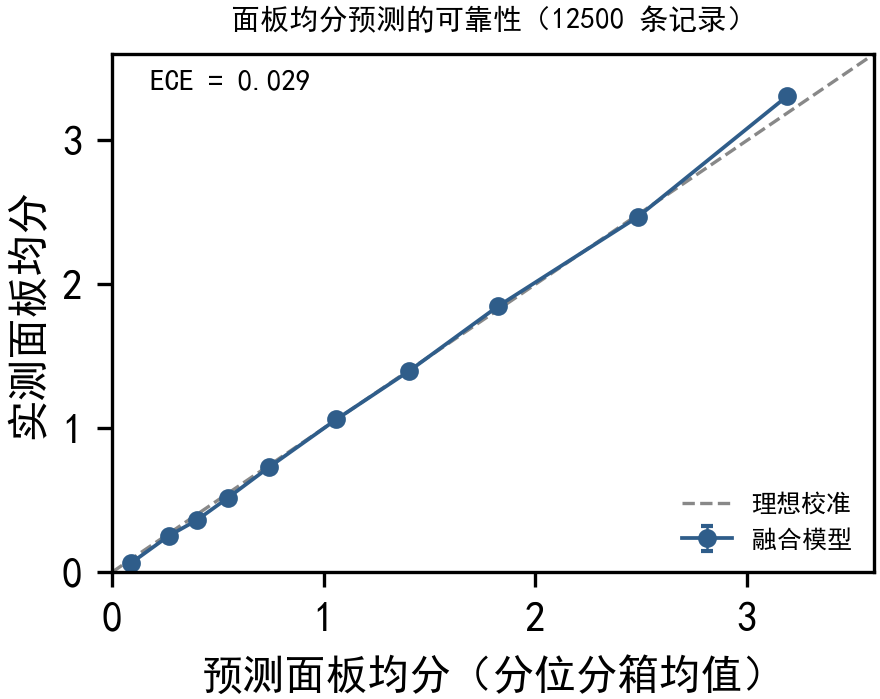
\includegraphics[width=0.92\columnwidth]{figures/fig13_calibration.png}
\caption{面板均分预测的可靠性曲线。十等分箱的实测均值基本落在对角线上，ECE 为 0.029；最高一箱（预测 3.19 分）低估 0.12 分，说明模型压缩了高分端。误差棒为一倍标准误。}
\label{fig:cal}
\end{figure}

逐目标看，最容易的是 \texttt{coriander}（0.108 分）与 \texttt{acetic}（0.166 分），最难的是 \texttt{A\_esters\_isoaa}（0.711 分）、\texttt{A\_esters\_ethac}（0.631 分）与 \texttt{A\_esters\_all}（0.620 分）。难的目标集中在酯类总量与乙酸酯，这类维度在风格间差异大、面板分歧也大，误差不是模型选错造成的。

两个汇总口径也会改变模型排名：核心 30 项上 ET 略好于 GBR（0.50589 对 0.50819），全 50 项上 GBR 反而更好（0.43780 对 0.44336）。单一口径的排名并不稳固，这也是本文同时报告两个口径、并用融合降低单模型波动的原因。

\begin{table}[t]
\centering
\small
\renewcommand{\arraystretch}{1.15}
\caption{七种方法的面板均分留出误差（单位：分）}
\label{tab:mae}
\begin{tabular}{@{}p{0.38\columnwidth}>{\centering\arraybackslash}p{0.27\columnwidth}>{\centering\arraybackslash}p{0.27\columnwidth}@{}}
\toprule
方法 & 核心 30 项/分 & 全 50 项/分 \\
\midrule
训练均值 & 0.60450 & 0.54879 \\
总体中位数 & 0.58785 & 0.52275 \\
风格中位数 & 0.50969 & 0.44712 \\
岭回归 & 0.52270 & 0.45708 \\
极端随机树 & 0.50589 & 0.44336 \\
梯度提升树 & 0.50819 & 0.43780 \\
固定等权融合 & 0.50222 & 0.43560 \\
\bottomrule
\end{tabular}

\vspace{0.3em}
{\footnotesize 注：留出预测为五次留出结果的平均，MAE 以酒为单位计算。}
\end{table}

\begin{figure}[t]
\centering
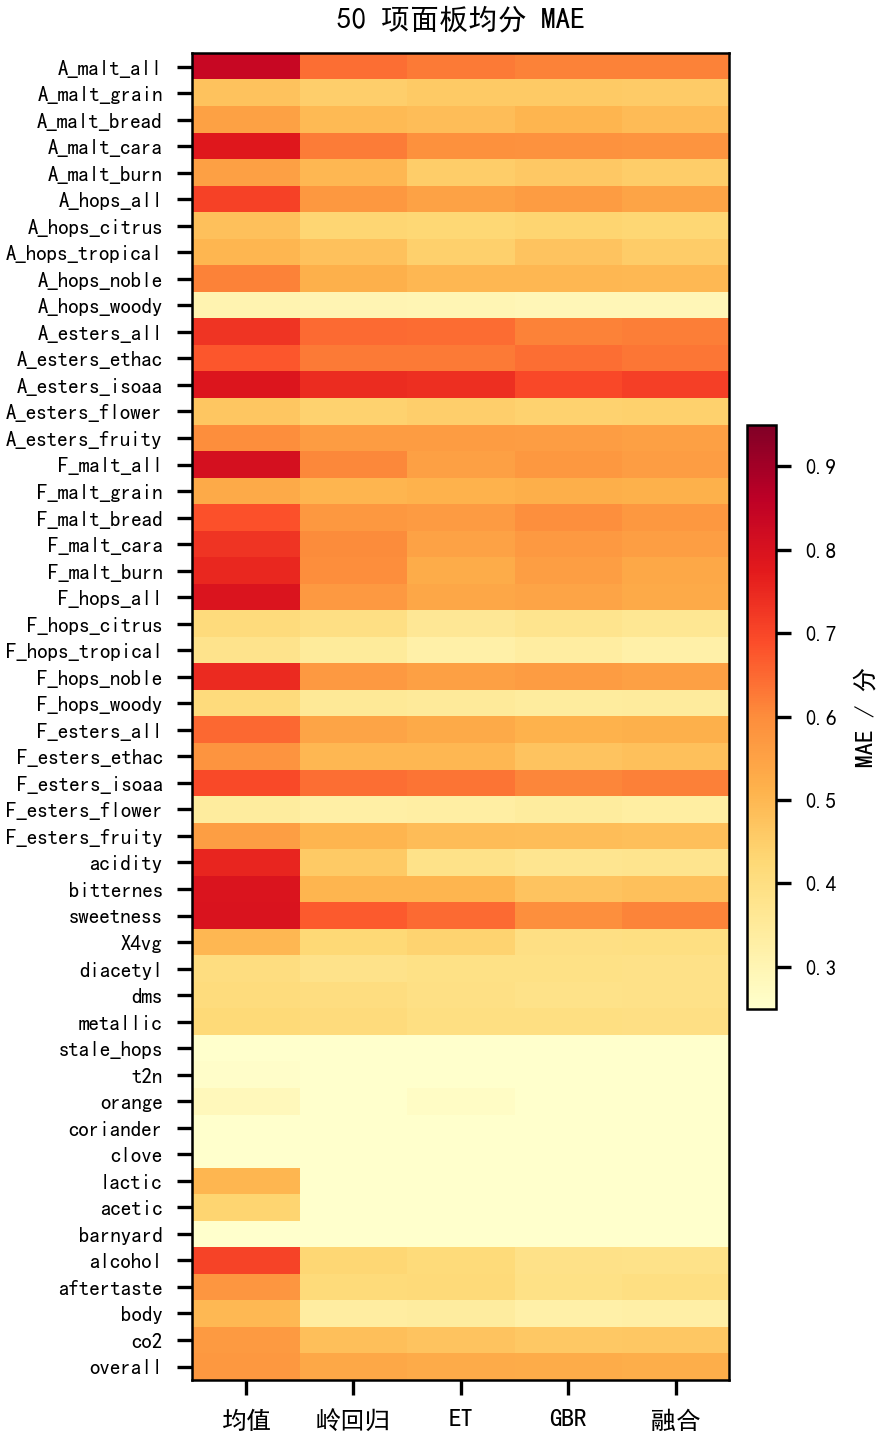
\includegraphics[width=0.95\columnwidth]{figures/fig05_error_heatmap.png}
\caption{50 项目标在 5 种模型下的留出 MAE。误差集中在低方差目标与口感类维度，模型差异只出现在少数目标。}
\label{fig:maeheat}
\end{figure}

\subsection{七级分布与等级识别}

七级分布模型在分布指标上优于两条基线，但总体一致率的提升几乎全部来自零等级；非零等级的识别仍是短板。

以第 3 节的七级分布 $q_{bjk}$ 为监督目标，用多输出极端随机树直接估计七维概率 $\hat p_{bjk}$，再取众数和中位数作为等级输出。表\ref{tab:ordinal} 比较三条路线：训练集的总体经验分布、训练折内的风格经验分布，以及频率极端随机树。三者使用同一套留出折与同一批 7500 条核心记录。

频率 ET 的 $D$ 为 0.02178，低于总体基线的 0.02820 和风格基线的 0.02313；期望 RPS 为 0.11044，低于总体基线的 0.11685 和风格基线的 0.11179。两项分布指标都优于两条基线，化合物信息确实带来改进。

但等级指标给出相反的画面：总体众数一致率 80.52\%，仅比总体基线的 79.31\% 高 1.21 个百分点，还低于风格基线的 80.72\%；非零众数一致率 24.33\%，低于风格基线的 26.58\%。这里出现了指标间的冲突：分布距离和期望 RPS 都支持频率 ET，等级一致率却支持风格基线。冲突的根源是评价对象不同——前两者衡量整条分布，后者只衡量概率最大的那一级；当零等级占近八成时，众数一致率对少数非零等级的错分不敏感。

分布指标改善而等级指标不改善，原因在零膨胀。核心 30 项的 7500 条记录中，观测众数为 0 的占 78.03\%，频率 ET 预测为 0 的占 81.29\%，多出 3.26 个百分点。总体一致率主要由“预测 0 且观测也是 0”撑起；只要把零等级判对，总体一致率就接近 80\%。

零膨胀下的类别不平衡会使总体一致率失真，这是分类评价中的常见现象\cite{hastie2009}。进一步对七个观测等级等权计算宏平均 F1 与平衡准确率，并报告有序等级平均绝对误差。本文保留总体一致率是为了与常规报告口径可比，但同时报告非零一致率，避免用一个被零等级主导的数字下结论。

只看非零记录，识别能力立刻暴露：1648 条观测众数非零的记录中，27.85\% 被预测成 0，只有 24.33\% 的预测等级与观测众数完全一致。属性之间的差异更大：\texttt{A\_hops\_noble} 的 49 条非零记录全部被预测为 0。图\ref{fig:conf} 的混淆矩阵显示，对角线以外的主要误差是把非零等级判为 0，总体一致率掩盖了这部分误差。

针对零膨胀，本文尝试过先判零、再估非零等级的两阶段模型：在与频率模型同为 32 棵树的条件下，非零众数一致率由 24.76\% 升到 25.49\%，提高 0.73 个百分点，但提高幅度的固定条件 95\% 区间 $[-0.91,2.30]$ 个百分点含 0，$D$ 也由 0.02178 升到 0.02200。表中 200 棵树的主模型非零一致率为 24.33\%，与 32 棵树对照的口径不同。证据不足以支持替换，主模型仍取频率 ET；这与 4.2 节的判断一致，化合物输入能修正分布的整体形状，却不足以改变具体等级的排序。

\begin{table}[t]
\centering
\footnotesize
\setlength{\tabcolsep}{1.5pt}
\renewcommand{\arraystretch}{1.15}
\caption{核心 30 项七级分布模型的比较}
\label{tab:ordinal}
\begin{tabular}{@{}p{0.28\columnwidth}>{\centering\arraybackslash}p{0.15\columnwidth}>{\centering\arraybackslash}p{0.15\columnwidth}>{\centering\arraybackslash}p{0.15\columnwidth}>{\centering\arraybackslash}p{0.15\columnwidth}@{}}
\toprule
方法 & $D$ & 期望 RPS & 众数一致率 & 非零一致率 \\
\midrule
总体分布基线 & 0.02820 & 0.11685 & 79.31\% & 21.30\% \\
风格分布基线 & 0.02313 & 0.11179 & 80.72\% & 26.58\% \\
频率 ET & 0.02178 & 0.11044 & 80.52\% & 24.33\% \\
\bottomrule
\end{tabular}

\vspace{0.3em}
{\footnotesize 注：$D$ 与 RPS 无量纲；非零一致率在观测众数非零的 1648 条记录上计算。}
\end{table}

\begin{table*}[t]
\centering\small
\caption{核心30项的留出众数等级补充评价}\label{tab:balanced}
\begin{tabular}{lrrrrr}
\toprule
方法 & 宏平均F1 & 平衡准确率 & 等级MAE & 总体一致率 & 非零一致率\\
\midrule
总体分布基线 & 0.2117 & 0.2490 & 0.4168 & 79.31\% & 21.30\%\\
风格分布基线 & 0.3352 & 0.3184 & 0.4020 & 80.72\% & 26.58\%\\
频率ET & 0.2855 & 0.2835 & 0.3912 & 80.52\% & 24.33\%\\
\bottomrule
\end{tabular}
\par\footnotesize 注：7500个酒—属性记录先合并再按七个实际出现的等级计算宏F1与召回均值；同一酒的30项并非独立观测。风格基线使用已知风格，各折只用训练酒的同风格评分分布。等级MAE按众数等级差计算。
\end{table*}

表\ref{tab:balanced}的平衡准确率和宏F1显示，频率ET低于已知风格基线，而等级MAE较低。三种指标关注的分类与等级距离不同；各方法使用相同外层留出酒和训练折构造基线，风格基线额外依赖风格标签，ET使用化学字段。结果支持保留多种端点及强基线，不支持仅用总体一致率概括非零等级能力。

\begin{figure}[t]
\centering
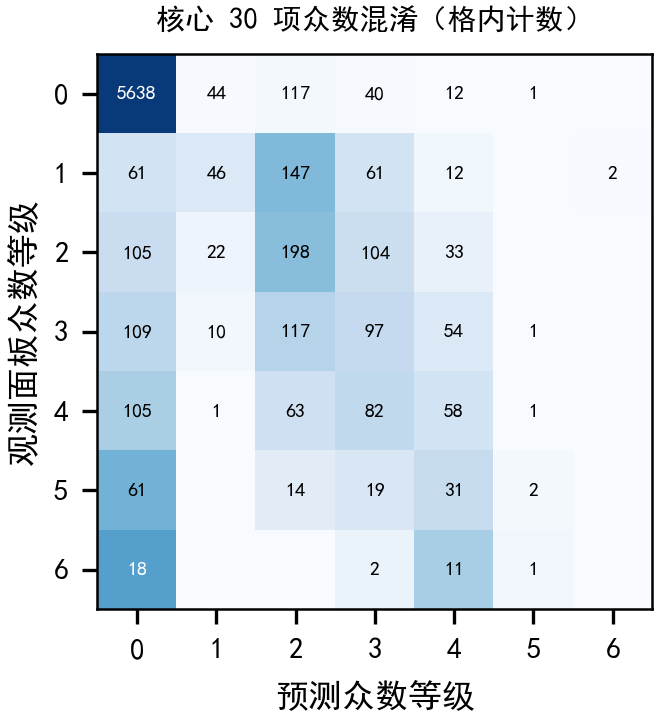
\includegraphics[width=0.95\columnwidth]{figures/fig06_confusion.png}
\caption{核心 30 项留出预测的面板众数等级混淆矩阵。零等级占据对角线的大部分计数，对角线以外的主要误差是把非零等级判为 0。}
\label{fig:conf}
\end{figure}

\subsection{预测区间与缺失条件下的鲁棒性}

保形区间在整体上达到名义覆盖，但在品评人数少的目标上明显不足；缺失机制比缺失比例更能解释性能下降。

区间用五次分割的保形预测构造\cite{lei2018}：每次 150 款酒训练、50 款酒校准、50 款酒测试，按属性在校准集上取绝对残差的分位数，得到该属性的固定半宽。五次分割的逐属性平均覆盖率为 90.06\%，平均宽度为 1.7342 分。覆盖率接近 90\% 的名义水平，说明边际校准是成功的。

保形预测只要求校准集与测试集可交换，不要求残差服从正态分布；按属性分别校准，也避免了跨属性的尺度差异。这两点是它适合面板均分的原因，但也意味着覆盖率是边际的，不是对每款酒、每个人数分组都成立。

边际覆盖不等于条件覆盖。按历史面板人数把测试记录分组，3—4 人组（12 款酒）覆盖率只有 74.00\%，5—7 人组为 86.89\%，8 人及以上组为 92.94\%，随人数单调上升。人少时面板均分本身的抽样噪声更大，而区间半宽按属性统一给出，没有随该酒的实际人数调整，于是小面板目标的残差更容易超出区间。图\ref{fig:cov} 同时给出分组覆盖与面板人数分布：3—4 人组覆盖明显偏低，说明“人少的目标区间不可信”。

分组覆盖的单调性同时给出了使用建议：对 3—4 人的酒样，应把区间宽度按人数放大，或直接标注覆盖不足；对 8 人以上的酒样，现有半宽偏保守，可以适当收窄。区间宽度目前按属性统一估计，尚未利用品评人数这一协变量。

缺失实验分两块。一块在测试阶段叠加完全随机缺失（MCAR），用训练阶段拟合的插补参数填补；15 折聚合下，核心 MAE 由 0.51086 升到 0.52662（20\% 缺失），众数一致率由 80.51\% 降到 80.33\%。这一块只回答随机丢数的代价，不覆盖系统性缺失。

另一块固定 3 折、重复 2 次，使用 300 棵树的 ET，基准 MAE 为 0.50666，分别施加 MCAR（10\%、20\%）、MAR（20\%）、整块通道缺失（20\%）和低值非随机缺失（MNAR，20\%）五个条件，结果见表\ref{tab:missing} 与图\ref{fig:missexp}。

同为 20\% 缺失比例，MNAR 低值条件的 MAE 增量为 $+0.02727$ 分，约为 MCAR 20\%（$+0.01393$）的两倍，也高于 MAR 20\%（$+0.01148$）；整块通道缺失的代价反而最小（$+0.00695$），约为 MCAR 20\% 的一半。缺失机制比缺失比例更重要：随机丢失只是减少信息量，系统性低值缺失还改变了“未检出”与“低浓度”的对应关系，插补会把缺失填向条件均值，模型因而失去区分低浓度样品的能力。同一条件下等级精确率由 0.5399 降到 0.5088，Spearman 相关由 0.4472 降到 0.3985，退化不限于均分。

四类机制的差别可以用缺失与取值的依赖关系解释。MCAR 下缺失与浓度无关，插补误差只来自信息减少；MAR 下缺失可由已观测变量解释，插补还能利用部分信息；整块缺失相当于删掉一个输入通道，剩余通道仍保留大部分信号，在 20\% 比例下代价最小；MNAR 低值缺失直接依赖未观测的低浓度，插补会把低值拉向条件均值，系统性偏差最大。

因此，题面所说的“数据缺失”不能只按缺失比例做压力测试：对仪器数据，低值缺失和整通道未测是两种不同的机制，前者对感官预测的伤害更大。两套缺失实验的基准不同：15 折 MCAR 压力的基准是 0.51086，新增机制实验的基准是 ET-300 的 0.50666，折数与模型设置都不同，两个基准不能直接相减。本文只在各自实验内部比较增量，避免把口径差异误读为机制效应。

\begin{table}[t]
\centering
\small
\renewcommand{\arraystretch}{1.15}
\caption{六种缺失条件下的核心 30 项 MAE 增量（单位：分）}
\label{tab:missing}
\begin{tabular}{@{}p{0.52\columnwidth}>{\centering\arraybackslash}p{0.34\columnwidth}@{}}
\toprule
缺失条件 & MAE 增量/分 \\
\midrule
无缺失 & 0 \\
MCAR 10\% & $+0.00656$ \\
MCAR 20\% & $+0.01393$ \\
MAR 20\% & $+0.01148$ \\
整块通道 20\% & $+0.00695$ \\
MNAR 低值 20\% & $+0.02727$ \\
\bottomrule
\end{tabular}

\vspace{0.3em}
{\footnotesize 注：基准为 ET-300 的 0.50666 分；增量为相对无缺失条件的差值。}
\end{table}

\begin{figure*}[t]
\centering
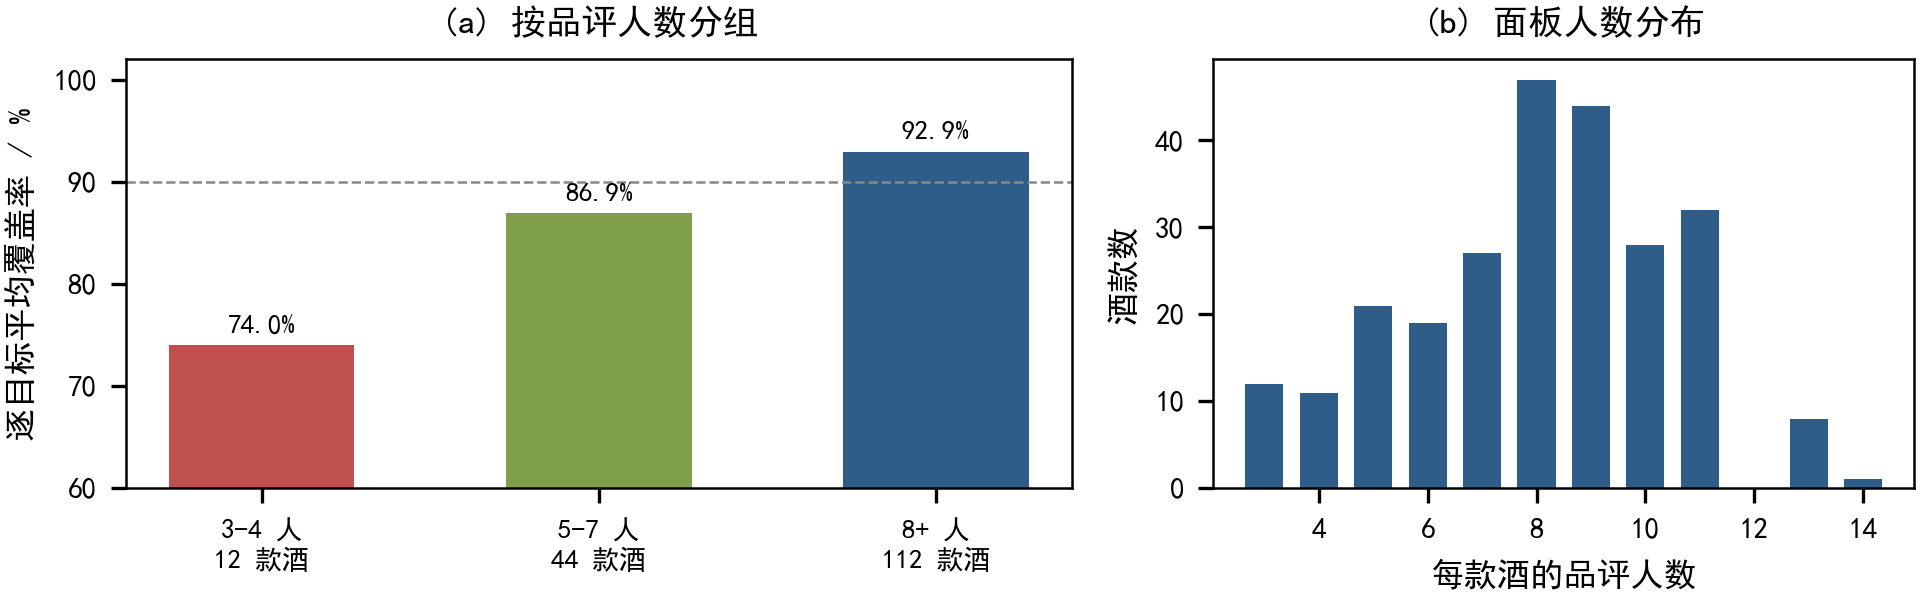
\includegraphics[width=0.95\textwidth]{figures/fig07_coverage.png}
\caption{按品评人数分组的保形区间覆盖率与面板人数分布。覆盖率随人数增加而上升，3—4 人组仅 74.00\%，边际覆盖不能保证小面板目标的条件覆盖。}
\label{fig:cov}
\end{figure*}

\begin{figure}[t]
\centering
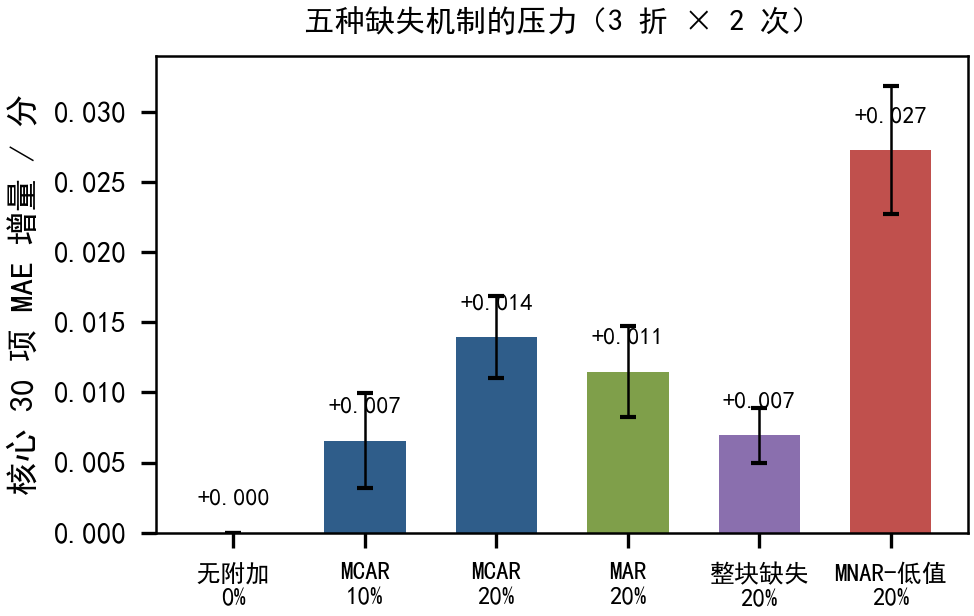
\includegraphics[width=0.95\columnwidth]{figures/fig08_missing_exp.png}
\caption{五种缺失条件下的核心 30 项 MAE 增量（基准 ET-300，0.50666）。系统性低值缺失的代价约为随机缺失的两倍；同为 20\% 时，整块通道缺失的代价最小。}
\label{fig:missexp}
\end{figure}

\subsection{讨论：风格信息与化学输入}

风格中位数基线在核心30项上达到0.50969分，融合模型为0.50222分，两者的固定留出预测重采样区间包含零。两者使用的信息不同：风格基线需要已知风格，融合模型使用化学字段；它们之间的误差差异不能分解为各类信息的独立贡献。

在同样获得风格标签的ET对照中，加入化学字段使核心MAE从0.51701降至0.50275，相对仅风格ET的固定预测重采样区间未跨零。这一结果表明化学字段在该模型和划分下提供了可用的预测信息；然而与风格中位数比较的区间跨零，不能概括成对所有风格基线都有稳定提升。新对照属于审查后的探索性实验，需用新酒样或预先确定的后续划分检验。

等级预测仍有明显短板。核心属性观测众数为0的比例为78.03\%，频率ET的总体一致率为80.52\%，非零众数一致率为24.33\%。宏平均F1、平衡准确率和等级MAE展示不同的模型排序，因而部署时应根据错判非零等级与等级距离的代价选择决策指标。逐属性和逐风格结果用于确定哪些目标需要补充数据或专门建模。

第二问的Top-3基于标准化岭回归系数筛选，并结合重采样与置换贡献分层；这些条件关联和相关网络不能直接解释为因果作用。第三问的生成画像沿用预测端点，其候选还需经过缺陷约束、独立训练代理与实际制备验证。

\section{第二问：化合物关联结构与关键因素}\label{sec:q2}

\subsection{共表达图的构建}

高相关只集中在少数化合物族，多数字段与其他字段近似独立，图正则能够影响的系数范围因此在建模之前就已受限。在 250 款酒的全部 231 个数值字段上计算 Spearman 秩相关，保留 $|r|\ge0.7$ 的字段对作为边，边权取带符号的相关系数，得到 231 个节点、109 条边。浓度字段跨越多个数量级且含截尾值，秩相关对单调变换不敏感，适合这种分布。有边的字段只有 81 个，其余 150 个字段没有任何邻居，约占全部字段的三分之二。

81 个非孤立字段被划为 19 个模块，最大模块含 15 个字段，109 条边的平均 $|r|$ 为 0.79，模块成员与化合物族基本对应。最大的两块以脂肪酸乙酯、乙酸酯和发酵综合量为主，包括乙酸乙酯、辛酸乙酯、癸酸乙酯、乙酸苯乙酯、乙醇、甘油与酯类总量；随后是酒花倍半萜烯氧化物（石竹烯氧化物、蛇麻烯环氧化物 II、$\alpha$-木罗醇等）、C$_6$—C$_9$ 高级醇（3-甲基-2-己醇、1-辛醇、4-甲基-1-戊醇等）与单萜醇（linalool、$\alpha$-松油醇、香茅醇）。酯类主要来自酵母的酯合成，酒花萜烯随酒花添加进入，高级醇是发酵副产物，模块因此沿原料与代谢途径分层；同类化合物共享前体与合成途径，这是高相关只出现在少数族内的化学原因。

109 条边全部为正相关，最小 $r$ 为 0.703，本数据中没有出现 $|r|\ge0.7$ 的负相关字段对。有符号权重保留了方法的一般性，但“负相关边鼓励系数反向”的机制未被触发，后文的图惩罚实际只做同向平滑。

图\ref{fig:net}(a) 把邻接矩阵按模块排序，非零元集中在少数对角块内，块外接近空白；图\ref{fig:net}(b) 给出模块规模，除前几个模块外，其余模块只含 2—3 个字段。同类化合物由同一原料或同一代谢途径产生，因而同向共变，这与以化合物谱预测复杂风味的既有结果一致\cite{schreurs2024}。孤立字段并非无关紧要，它们只是缺少 $|r|\ge0.7$ 的强共变伙伴，其系数只能由自身与目标的关系决定；孤立字段的拉普拉斯行恒为零，图惩罚只能在 81 个字段内部传递信息。

以上网络在全部数据上估计，用于描述。

阈值决定图的疏密。把 $|r|$ 的门槛由 0.6 提到 0.9，边数从 266 条降到 9 条，非孤立字段从 130 个降到 15 个（表\ref{tab:threshold}）。0.7 是折中：再低会把经由第三变量产生的间接关联连进来，模块结构被稀释；再高只剩 9 条边，94\% 的字段成为孤立点，图惩罚几乎无处可施。0.7用于全数据网络的描述；模型验证时在每个训练折重算相关图，并在内层候选阈值0.6、0.7、0.8中选参。

\begin{table}[t]
\centering\small\renewcommand{\arraystretch}{1.15}
\caption{相关阈值对网络结构的影响（231 个字段）}
\label{tab:threshold}
\begin{tabular}{@{}cccc@{}}
\toprule
阈值 $|r|$ & 边数 & 连通分量 & 孤立字段 \\
\midrule
0.6 & 266 & 114 & 101 \\
0.7 & 109 & 169 & 150 \\
0.8 & 39  & 207 & 194 \\
0.9 & 9   & 222 & 216 \\
\bottomrule
\end{tabular}
\end{table}
建模时相关图在每个训练折内单独重算，测试折不参与，图结构与评价样本保持分离。

\begin{figure*}[t]
\centering
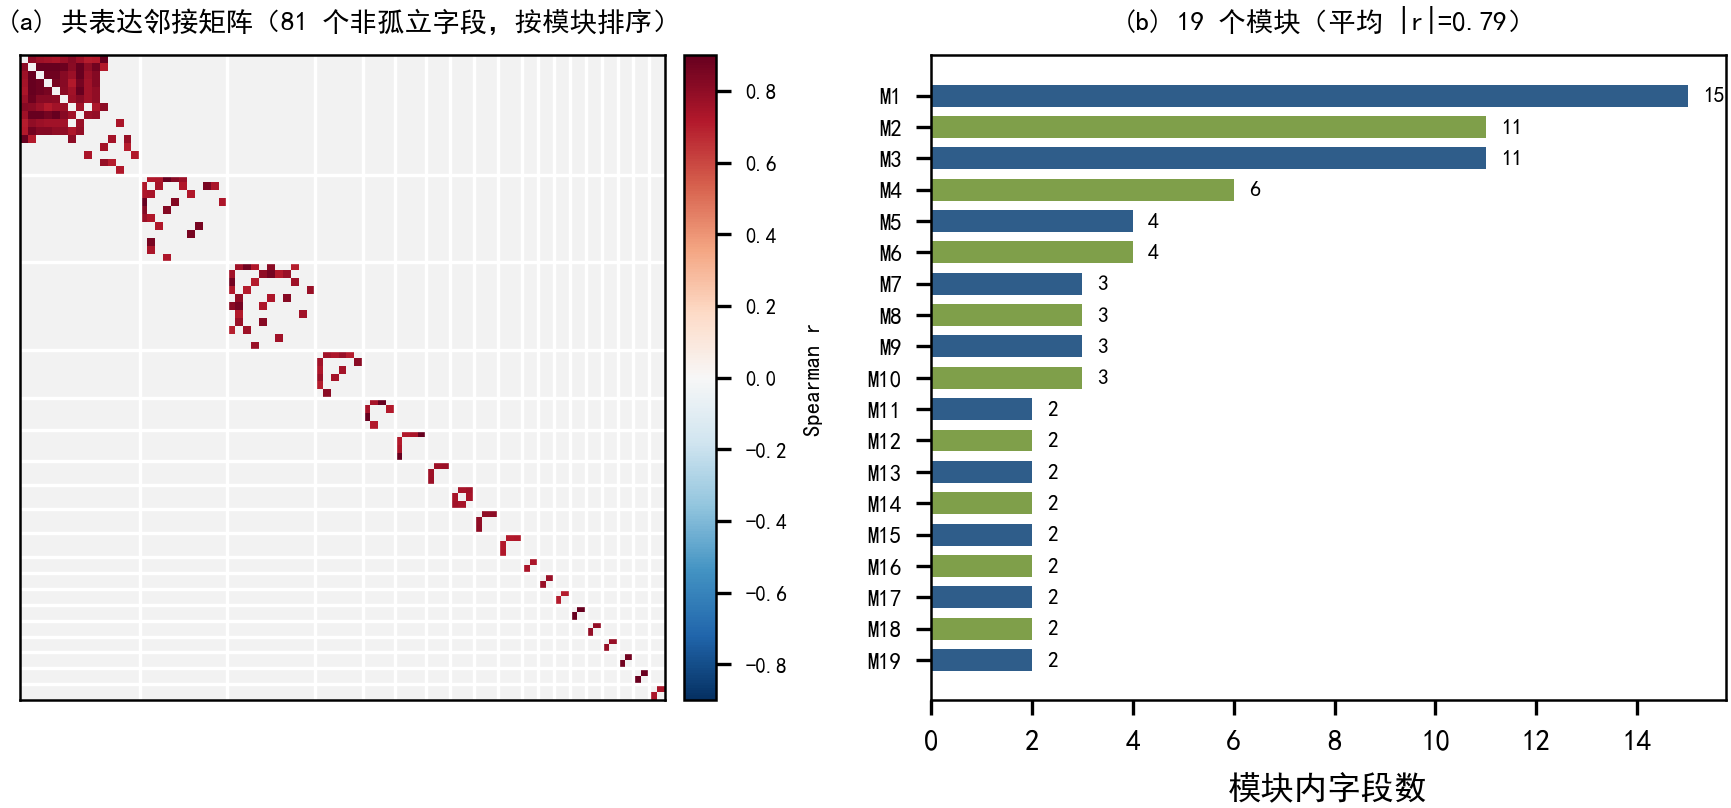
\includegraphics[width=0.98\textwidth]{figures/fig09_network.png}
\caption{共表达网络的结构。(a) 81 个非孤立字段的邻接矩阵按模块排序，非零元集中于少数对角块，块外基本空白；(b) 19 个模块的规模，除前几个模块外均只含 2—3 个字段。}
\label{fig:net}
\end{figure*}

\subsection{图约束模型与可解性}

图约束模型在 $\alpha>0$、$\lambda\ge0$ 时严格凸、解唯一，三种图设定之间的误差差异因此来自惩罚项中的图结构，而不是求解过程。

记标准化后的化合物矩阵为 $Z\in\mathbb{R}^{250\times231}$，中心化后的感官均分矩阵为 $Y_c\in\mathbb{R}^{250\times50}$，待估系数矩阵为 $B\in\mathbb{R}^{231\times50}$。图用带符号权重矩阵 $W$ 表示，拉普拉斯矩阵取 $L=\operatorname{diag}(\sum_j|W_{ij}|)-W$，模型为

\begin{equation}
\begin{aligned}
\hat{B}=\arg\min_{B}\Bigl\{&\|Y_c-ZB\|_F^2+\alpha\|B\|_F^2\\
&+\lambda\operatorname{tr}(B^{T}LB)\Bigr\}.
\end{aligned}
\label{eq:graph}
\end{equation}

式\eqref{eq:graph} 的第一项是拟合误差，第二项是岭惩罚，第三项让正相关邻边的系数接近、负相关邻边的系数方向相反；$\lambda=0$ 时模型退化为普通岭回归。$\lambda$ 增大时，系数更受带符号邻边的约束；若负边构成符号不平衡的环，图惩罚的零空间不必保留每个分量的一个自由度。$\alpha$ 控制整体收缩的强度，$\lambda$ 控制沿边差异的强度，两者共同决定模型的有效自由度，这也是二者需要在折内同时选择的原因。

对任一系数向量 $b$，有

\begin{equation}
b^{T}Lb=\sum_{i<j}|W_{ij}|\left(b_i-\operatorname{sign}(W_{ij})b_j\right)^2\ge0.
\label{eq:psd}
\end{equation}

式\eqref{eq:psd} 可由 $b^{T}Lb=\sum_i\sum_j|W_{ij}|b_i^2-2\sum_{i<j}W_{ij}b_ib_j$ 逐项配方得到。右边每个平方项非负，故 $L$ 半正定；等号成立当且仅当在 $W$ 的每个连通分量内 $b_i=\operatorname{sign}(W_{ij})b_j$，即系数沿边的符号保持一致。

由式\eqref{eq:psd}，$\lambda$ 项是 $B$ 的凸函数；$\alpha>0$ 使 $\alpha\|B\|_F^2$ 的 Hessian 为 $2\alpha I$，目标函数强凸，式\eqref{eq:graph} 因而有唯一解。等价地，正规方程 $(Z^{T}Z+\alpha I+\lambda L)B=Z^{T}Y_c$ 的系数矩阵正定。若 $\alpha=0$，带符号 $L$ 的零空间由各边的符号约束决定，唯一性取决于 $Z$ 与 $L$ 的共同零空间；本文字段存在强共线，正岭惩罚因此不可省去。50 个目标共享同一个 $L$，惩罚不跨目标耦合，每个目标等价于一个单独的正则回归；图只改变同一目标内部不同字段的系数分配，不改变目标之间的相对难度。

参数与外层评价严格分离：$\alpha$、$\lambda$ 与相关阈值都在每个训练折内部由内层留出误差选择，外层测试折不参与；同一折内另取 10 个节点标签随机置换的图，按相同流程重建并重新选参，作为结构无关的零模型。零模型也经过调参，误差中包含选择波动，比较时按同一协议解读。图结构回归的惩罚形式取自图结构变量的回归与选择\cite{li2010}。

\subsection{双口径结果}

真实图的差值随评价口径变号：单折口径比无图差0.000124分，五次预测聚合后好0.001283分。结合效应量和最终全数据选参，现有证据不支持图正则具有稳定且实际意义明确的预测优势；网络主要用于描述化学共变结构。

两种口径评价不同对象。单折口径把 15 个外层折的留出 MAE 再平均，每次拟合只产生一次预测，对应“训练一次即上线”的误差；聚合口径先对同一款酒的五次留出预测取平均，再在 250 款酒上计算 MAE，对应“重复建模、预测取均值”的误差。前者的样本单位是折，后者是酒；前者保留单次拟合的方差，后者通过平均削去一部分方差。同一批预测在两种口径下给出相反符号，说明图的效应与汇总方式有关，不能脱离口径单独陈述；两种口径对应不同的部署假设，并列报告才能覆盖两种使用场景。

表\ref{tab:graph} 给出核心 30 项的结果。单折平均为无图 0.536911、真实图 0.537035、打乱图 0.537794；聚合预测为无图 0.526148、真实图 0.524865，差值 $-0.001283$，固定预测条件下以酒为单位重采样2000次的 95\% 区间为 $[-0.002341,-0.000229]$。该区间以固定留出预测为条件，不包含重训与选参的不确定性；区间未跨0，但误差差值仅0.001283分，实际意义需要结合任务精度判断。

\begin{table*}[t]
\centering\small\renewcommand{\arraystretch}{1.2}
\caption{核心 30 项在图模型三种设定下的 MAE}
\label{tab:graph}
\begin{tabular}{@{}lcccc@{}}
\toprule
评价口径 & 无图 & 真实图 & 打乱图 & 真实图减无图 \\
\midrule
单折平均（15 个外层折） & 0.536911 & 0.537035 & 0.537794 & $+0.000124$ \\
聚合预测（按酒平均） & 0.526148 & 0.524865 & — & $-0.001283$ \\
\bottomrule
\end{tabular}
\end{table*}

打乱图作为结构对照，在单折口径下平均误差最高；该结果本身不能分离随机图平滑和选参造成的差异。真实图与无图的差距很小。效应小有结构性原因：150 个字段是孤立节点，其系数行不受图惩罚；15 个外层折中只有 7 折选到正的 $\lambda$，其余 8 折的 $\lambda=0$，模型退化为岭回归。图只在不到一半的折里对 81 个字段中的一部分起作用，最优强度在多数折内被内层准则判为零。

聚合口径把每款酒的五次预测平均。重复划分的训练集相互重叠，五次预测存在相关性，平均后的方差不能假定缩减至五分之一；本实验没有分解图惩罚对偏差与方差的影响。

全 50 项的单折结果为无图 0.470061、真实图 0.470220、打乱图 0.471037，排序与核心 30 项一致，差异同样在万分位。 最终描述模型由全部数据上的三折内层验证按核心30项MAE选择参数，重算网格中 $\alpha=1000,\lambda=0$ 的内层误差为0.539083；最佳正图惩罚组合为 $\alpha=1000,\lambda=1,\tau=0.8$，误差为0.539086。选参依据是内层误差和既定网格排序，不是使用外层聚合误差或重采样区间直接选取 $\lambda$。最终用全部数据拟合的描述模型选得 $\lambda=0$，Top-3 由岭回归系数给出。图在本文中承担解释功能，不是预测模型的组成部分；把它写成“提升了预测精度”会与最终选择矛盾。

\subsection{Top-3 的稳定性}

150 条候选中只有 36 条同时满足频率、折数与置换贡献三项条件；Top-3 对单元格级异常稳健，对变量集合敏感，因此不能读作变量选择结论。

对 50 个目标各取标准化岭回归系数绝对值最大的 3 个字段，共 150 条记录。以酒为单位做 200 次 bootstrap，同一款酒的各目标一起进出，目标间的相关性不被打破；每次重建预处理与相关图，并固定全数据选定的 $\alpha$、$\lambda$ 与阈值，记录字段是否仍在该目标的前三位，得到入选频率\cite{efron1993}；同时统计 15 个外层折中的入选次数，以及留出数据上普通置换与风格内置换的误差增量。支持条件为频率不低于 0.5、至少在 5 个外层折入选、两种置换的平均贡献均为正，三项分别对应重采样稳定性、跨折稳定性与预测贡献。

单看频率有 46 条不低于 0.5，且都至少在 5 折入选；再要求两种置换贡献为正，剩 36 条，被剔除的 10 条都是置换贡献不稳定的记录。36 条候选分布在 29 个目标上：22 个目标各 1 条、7 个目标各 2 条，其余 21 个目标没有任何候选通过。图\ref{fig:top3}(a) 给出 150 条候选的入选频率分布，0.5 的门槛把候选分成通过与否两组，0.2—0.4 区间仍聚集了相当一部分记录，这些字段只是偶尔进入前三；图\ref{fig:top3}(b) 按目标给出通过比例，空白目标即没有候选通过。频率以固定参数为条件；若在每次重采样中重新选参，评估的是完整选择流程的稳定性。0.5 是本文采用的描述性门槛，不是显著性水平，门槛附近的频率差别不宜过度解读。

\begin{figure*}[t]
\centering
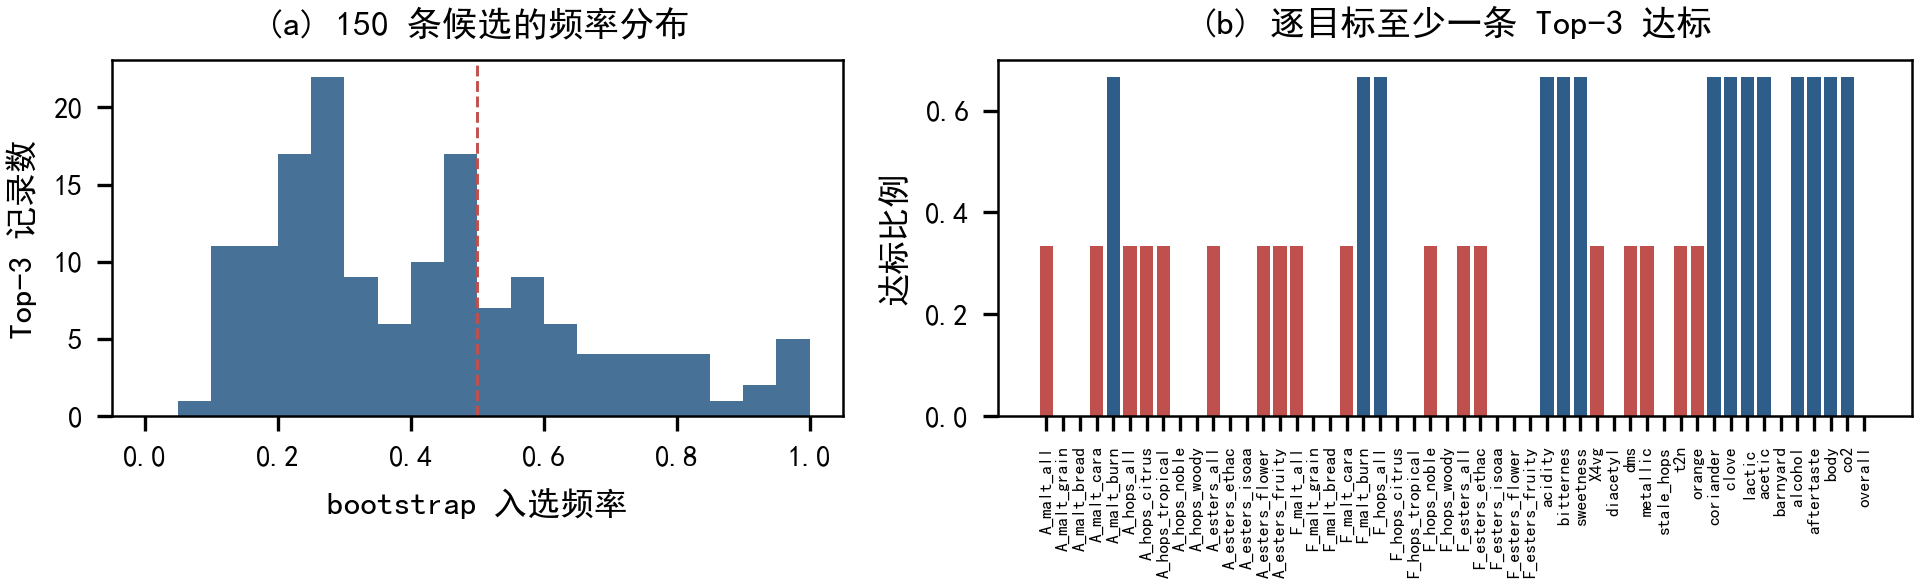
\includegraphics[width=0.98\textwidth]{figures/fig10_top3.png}
\caption{Top-3 的稳定性。(a) 150 条候选的 bootstrap 入选频率分布，虚线为 0.5 的门槛；(b) 逐目标通过支持条件的候选比例，空白目标表示没有候选通过。}
\label{fig:top3}
\end{figure*}

化学异常敏感性见表\ref{tab:top3}。把 80 个异常单元格置为缺失、仅用训练折估计填补后，核心 30 项 MAE 由 0.50641 变为 0.50691，全 50 项由 0.44478 变为 0.44515，预测值平均绝对变化 0.00500 分，Top-3 平均保留 97.64\%。仅使用第\ref{sec:scale}节所定义的 $V$（38个逐点一致字段、61个单位登记字段及226个非综合字段的交集）时，固定 $\alpha=1000$ 的15折岭回归 Top-3 平均保留36.18\%。该 $V$ 与含80处异常的32个字段完全不同，交集为空。

\begin{table*}[t]
\centering\small\renewcommand{\arraystretch}{1.2}
\caption{Top-3 的支持条件与化学异常敏感性}
\label{tab:top3}
\begin{tabular}{@{}lcc@{}}
\toprule
检验项目 & 数值 & 备注 \\
\midrule
通过支持条件的记录 & 36 / 150 & 频率$\ge0.5$、$\ge5$ 折入选、置换贡献为正 \\
核心 30 项 MAE（异常置缺失前 $\to$ 后） & 0.50641 $\to$ 0.50691 & 分 \\
全 50 项 MAE（异常置缺失前 $\to$ 后） & 0.44478 $\to$ 0.44515 & 分 \\
预测值平均绝对变化 & 0.00500 & 分 \\
Top-3 平均保留（异常置缺失） & 97.64\% & — \\
Top-3 平均保留（仅交集 $V$ 的32字段） & 36.18\% & — \\
\bottomrule
\end{tabular}
\end{table*}

两类扰动都改变输入，性质不同。前者只抹掉 80 个单元格，受影响字段仍由其余酒样支撑，系数排序几乎不动；后者把226个非综合字段压到交集 $V$ 的32个字段，候选池本身换掉，Top-3 只剩约三分之一。稳定的 Top-3 是“在当前字段集合与当前模型下稳定”，不是变量选择结论；换一套输入，排名会重排。

\subsection{化学解释及其边界}

三个例子分属三种证据强度：同名端点上的近确定性关联、机制清楚但经由未观测过程的关联、文献支持而统计支持不足的关联。系数、相关与入选频率都是关联量，单独任何一项都不构成因果证据。

X4VG 与 X4vg 的关系最强。X4VG 在该端点上的入选频率为 1.00，15 个外层折全部入选，系数为正。4VG 是阿魏酸经酵母脱羧的产物，赋予丁香与酚类香气，储藏中会下降并转化为香草醛等物质\cite{vanbeneden2008}。这一条的证据链最完整，但端点本身以该化合物命名，关联接近定义对应，属于模型复现命名关系，而不是独立发现。

iron 与 metallic 的关系次之。iron 在 metallic 上的入选频率为 0.94，15 个外层折全部入选，系数为正。铁不是香气化合物，金属感来自口腔中脂质氧化与铁离子的催化过程\cite{omur2012}；模型看到的是铁含量高的酒更容易被评出金属感这一共变，催化链本身没有进入模型。铁还与水质、设备与风格相关，当前设计无法把铁从这些过程变量中分离。iron 同时进入酒花香气、苦味与甜味等性质不同的端点，这种跨端点重复更像风格或工艺的代理变量，而不是某一感官属性的专属因素。

linalool 与 coriander 的关系最弱。linalool 以 0.46 的频率列第三，低于 0.5 的门槛，只在 8 个外层折入选。芫荽籽是小麦啤酒的传统香料，其添加阶段与用量会改变啤酒中的 linalool 含量\cite{pater2024}，文献给出的来源关系与正系数方向相容，但统计支持没有过线。文献支持与重采样稳定性是两个独立维度，前者不能替代后者。置换贡献衡量字段取值对留出误差的作用，贡献为正只说明该字段携带预测信息，不说明它通过化学途径影响感官。

共线化合物会在系数上互相替代。同一模块内的字段通过 $|r|\ge0.7$ 的边直接或间接相连，相关变量可能在系数排序中相互替代；模块级联合置换结果提供补充证据，但不能预设所有模块的系数和都稳定。可信的解释应落在模块层面，例如酒花倍半萜烯氧化物或脂肪酸乙酯这样的族，单个化合物名称只作为该族的代表。按模块报告时，“该族整体为正”与“族内某个化合物排名靠前”需要分开陈述，前者对共线替代不敏感。附件 8 的 GBM SHAP 与 MDI 来自原始研究的模型，本文只将其作为外部参照核对化学方向，不计入本队结果\cite{lundberg2017}。可检验的解释顺序是：先看模块是否与原料或工艺对应，再看代表化合物的方向与文献是否一致，最后用独立批次验证。

% 第三问：风格生成与迁移可行域

\section{第三问：风格生成与迁移可行域}\label{sec:q3}

第三问要做两件性质不同的事：在给定风格下生成新的化合物—感官谱，以及判断一款现有酒能否改造成目标风格。本文把二者拆成生成层与判别层：生成层回答哪种采样最像真实酒，判别层回答哪条改造路径在化学上站得住。总的判断是，生成质量无法用单一指标排序；迁移可行域主要由 DMS 与反式-2-壬烯醛卡住，且对阈值高度敏感。

\subsection{风格条件生成与评价体系}

生成质量在不同评价维度上会给出相反的排序，因此本文的生成体系从一开始就把分布接近与分类器认可分开记录。三个角色的划分互不重叠，是为了让生成器用过的酒不出现在评价里：生成器只用 G，评价器只用 J，真实参考只用 T。同一批 250 款酒在五次划分中被重复使用，因此后文的比较都是划分内比较，不构成外部验证。

生成对象取 Tripel（28 款）、Kriek（10 款）与 Lambic（11 款）。前者的样本量足以支撑 40 条谱的分布比较，后两者稀少，正好用来观察少样本风格上的退化；三个风格的样本量跨度覆盖了够用与不够用两种情形。每次划分把 250 款酒分成互不重叠的 G（生成器训练，100 款）、J（评价器训练，100 款）与 T（留出检验，50 款）；四种方法在每种风格上各生成 40 条谱，五次划分合计 2400 条。生成器只看到 G 中该风格酒样的 226 个非聚合化学字段。Kriek 与 Lambic 每划分进入 G 的只有 4 至 5 款、进入 T 的真实参考只有 2 款，Tripel 则为 11 款与 6 款，这一不对称决定了后文的读数方式。

四种方法对应四种关于配方空间的假设。重采样有放回地抽取 G 中的同风格酒样，不学习任何结构，是必须被击败的基线\cite{efron1993}；它不产生新组合，却是唯一保证生成点落在真实数据流形上的方法，任何生成器若在分布距离上赢不过它，就说不上学到了结构。局部凸组合假定新配方落在同风格近邻的连线上：
\begin{equation}
x_{\mathrm{new}}=u\,x_{a}+(1-u)\,x_{b},\qquad 0\le u\le 1,
\label{eq:convex}
\end{equation}
其中 $x_a,x_b$ 为 G 中同风格的两个酒样。凸组合对应配比微调这一工艺动作，生成点不会超出数据支撑。受约束局部凸组合在 \eqref{eq:convex} 之上要求生成点到最近同风格训练样本的距离不超过留一支撑半径，并在对数尺度上混合 DMS 与 4VG、裁剪到上下界。条件 PCA 高斯在 G 的风格内做主成分分解后于主成分空间拟合对角高斯并采样，允许生成点离开凸包，更容易产生训练集中没有的组合。

评价从生成器外部取四个角度。分布距离用固定训练带宽的 RBF 核最大均值差异 $\mathrm{MMD}^2$\cite{gretton2012}，真实参考为 T 中该风格酒样的非缺失测量；KS 统计量逐字段计算后取均值，刻画边缘分布的平移；精确复制比例统计与 G 中某训练点距离小于 $10^{-8}$ 的生成谱占比；独立评价器是只在 J 上训练的风格分类器，报告它赋予目标风格的平均概率与判为目标风格的比例。四项指标共用同一套预处理与核带宽，尺度差异不会被误读成分布差异。KS 只看单字段的边缘分布，对字段之间的相关性不敏感；$\mathrm{MMD}^2$ 在多维表示上一次比较整个联合分布，两者一起看才能区分单字段偏移与整体结构偏移。

分类器识别率高与分布更接近是两件不同的事。分类器只关心生成点落在决策边界哪一侧，对风格内部的协方差、尾部厚度与稀有组合不敏感；$\mathrm{MMD}^2$ 关心整个分布在再生核空间中均值嵌入的位置，对生成物挤向风格中心这类退化格外敏感。一种方法完全可以把样本堆到最典型的 Tripel 附近换来高识别率，同时因丢掉离散度而让 $\mathrm{MMD}^2$ 变大。本文因此不设综合评分，只并列报告四个维度。

\subsection{生成结果}

四种方法在三个风格上互有胜负，没有一种全面占优；重采样在分布距离上仍是难以击败的基线，但它的精确复制比例恒为 1。

\begin{table*}[t]
\centering
\caption{三种风格下四种生成方法的分布距离、边缘偏移、复制比例与独立评价器判断（五次划分平均；$\mathrm{MMD}^2$ 与 KS 越小越好，复制率为与训练点完全重合的生成谱比例，后两列由只在 J 上训练的分类器给出）}
\label{tab:gen}
\small
\begin{tabular}{llrrrrr}
\toprule
风格 & 方法 & $\mathrm{MMD}^2$ & KS 均值 & 复制率 & 评价器概率 & 判为目标风格 \\
\midrule
Tripel & 重采样 & 0.1034 & 0.4245 & 1.00 & 0.2992 & 0.565 \\
       & 局部凸组合 & 0.1135 & 0.4448 & 0 & 0.3432 & 0.755 \\
       & 受约束局部凸组合 & 0.1158 & 0.4463 & 0 & 0.3358 & 0.695 \\
       & 条件 PCA 高斯 & 0.1088 & 0.4605 & 0 & 0.1499 & 0.285 \\
\midrule
Kriek  & 重采样 & 0.2871 & 0.6208 & 1.00 & 0.5275 & 0.800 \\
       & 局部凸组合 & 0.3005 & 0.6511 & 0 & 0.5779 & 0.955 \\
       & 受约束局部凸组合 & 0.2988 & 0.6422 & 0 & 0.5703 & 0.950 \\
       & 条件 PCA 高斯 & 0.2832 & 0.6307 & 0 & 0.3101 & 0.595 \\
\midrule
Lambic & 重采样 & 0.2226 & 0.6257 & 1.00 & 0.4924 & 0.885 \\
       & 局部凸组合 & 0.2206 & 0.6602 & 0 & 0.5543 & 0.975 \\
       & 受约束局部凸组合 & 0.2181 & 0.6453 & 0 & 0.5598 & 0.995 \\
       & 条件 PCA 高斯 & 0.2095 & 0.6324 & 0 & 0.2091 & 0.385 \\
\bottomrule
\end{tabular}
\end{table*}

表\ref{tab:gen} 汇总五次划分的平均结果。Tripel 上受约束局部凸组合的识别率 0.3358 高于重采样的 0.2992，判为 Tripel 的比例 0.695 也高于 0.565，但它的 $\mathrm{MMD}^2$ 为 0.1158、KS 均值 0.4463，两项都劣于重采样的 0.1034 与 0.4245。同一风格上出现了方向相反的评价：按判别边界看受约束凸组合更像目标风格，按分布看重采样离真实酒样更近。重采样在两个距离指标上同时最好，说明它逼近真实分布靠的是直接复制，而不是学到了结构。约束没有换来指标收益，无约束版本的 $\mathrm{MMD}^2$ 为 0.1135、识别率 0.3432，两项都略好；约束的作用是保证生成谱不越界。

反向的例子同样清楚。条件 PCA 高斯在 Tripel 上的 $\mathrm{MMD}^2$ 为 0.1088，仅次于重采样，但独立评价器给它目标风格的概率只有 0.1499、判为目标风格的比例 0.285，两项都最低。这可能与对角高斯忽略主成分之间的相关性、生成点向风格中心收缩有关，结果是谱形趋于平均、反而越过分类边界。距离近而识别率低与识别率高而距离远，指向同一件事：两个指标度量的不是同一个东西。

Kriek 与 Lambic 上的距离整体大了一倍，落在 0.21 至 0.30 之间，四种方法都没有把这两个稀薄风格学到可用程度，而每划分只有 2 款留出酒，抽样误差不可忽略。这两个风格的化学谱离散度大、样本又少，40 条生成谱难以覆盖其变异范围。KS 在 Tripel 上集中在 0.42 至 0.46，在 Kriek 与 Lambic 上集中在 0.62 至 0.66；逐字段取平均会稀释单字段的尾部偏离，因此 KS 更适合判断整体平移，不适合判断尾部风险。Kriek 上条件 PCA 高斯最低（0.2832），重采样 0.2871；Lambic 上条件 PCA 高斯 0.2095、受约束凸组合 0.2181、重采样 0.2226，三者相差不足 0.014，识别率却相反，条件 PCA 高斯只有 0.2091。这两个风格上的读数只能支持重采样没有被稳定击败，不能支持任何方法的优越性。

覆盖度从另一侧约束生成质量。对每个真实酒样，计算它到最近生成点的标准化欧氏距离，再除以它到最近真实酒样的距离，得到相对覆盖比；比值小于 1 说明生成集把真实样品包住了。重采样最小（0.60--0.70），两种凸组合居中（0.61--0.73），条件 PCA 高斯最差（0.87--0.93），见表\ref{tab:coverage}。这解释了第二节的悖论：条件 PCA 高斯在 Kriek 与 Lambic 上 $\mathrm{MMD}^2$ 最低，并不是更贴近真实酒样，而是生成点偏离训练支撑、把分布拉宽，因而在核均值嵌入上"看起来"更接近。三项指标合起来才有完整判断：重采样保真且覆盖最好，但复制率为 1、不产生新组合；凸组合产生新组合、覆盖尚可，分布距离略差；条件 PCA 高斯覆盖最差。

\begin{table}[t]
\centering\small\renewcommand{\arraystretch}{1.15}
\caption{生成集的相对覆盖比（真实酒样到最近生成点距离 / 到最近真实酒样距离）}
\label{tab:coverage}
\begin{tabular}{@{}lccc@{}}
\toprule
方法 & Tripel & Kriek & Lambic \\
\midrule
重采样 & 0.698 & 0.653 & 0.600 \\
局部凸组合 & 0.729 & 0.648 & 0.606 \\
受约束局部凸组合 & 0.711 & 0.655 & 0.634 \\
条件 PCA 高斯 & 0.919 & 0.874 & 0.933 \\
\bottomrule
\end{tabular}
\end{table}

复制率给出了最干净的分界：重采样恒为 1，两种凸组合与条件 PCA 高斯恒为 0。复制率为 1 意味着每条生成谱都是训练集中已有的酒，作为生成新配方没有提供新组合，这正是重采样距离更近却不适合交付的原因。凸组合的复制率为 0，说明它们给出的是新的配比组合，代价是可能落在真实酒样稀疏的区域。

\begin{figure*}[t]
\centering
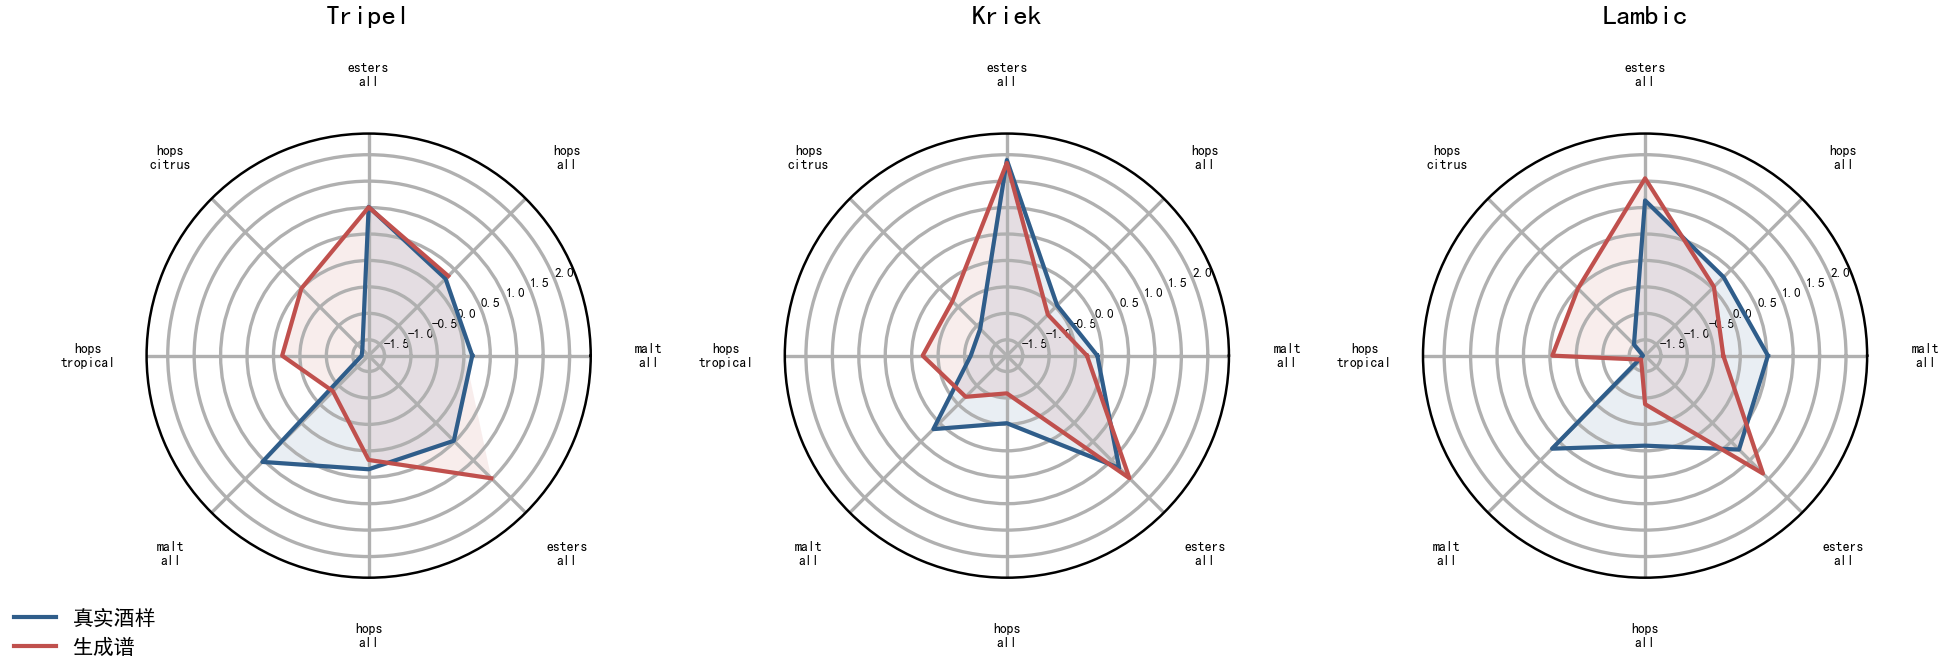
\includegraphics[width=0.98\textwidth]{figures/fig11_generation.png}
\caption{三种风格的真实酒样与生成谱在 8 个标准化感官维度上的相对强度。纵轴为按 8 维标准化后的相对强度，可正可负，因此比较的是曲线形状而不是绝对得分；生成谱的感官画像由第一问的预测模型给出，是预测值而非新酿酒的实测评价。}
\label{fig:gen}
\end{figure*}

图\ref{fig:gen} 的曲线在形状上大体重合，没有整体平移或维度错位，差异集中在酒花与麦芽两族维度，说明凸组合把邻近样本的谱形带了进来。

\subsection{迁移搜索与冻结候选}

迁移的可行性在三个证据层级上依次衰减，搜索可行只是最弱的一层。

迁移任务给定一款 Pils/Lager 源酒，问能否通过调整配比把它推到 Tripel。候选由源酒与 G 内每个 Tripel 锚点之间的线性插值生成，每个锚点取 30 档权重，逐点裁剪回给定上下界；每条记录由此产生 30 档乘锚点数的候选，绝大多数会在下一步被淘汰。筛选条件有五条：标准化空间的均方根改动不超过半径 1；到最近 Tripel 训练点的距离不超过其留一支撑半径；目标风格概率不低于 0.5，且比源酒与仅裁剪对照高出 0.01；四项缺陷不增；两个 G 感官模型给出的 stale hops 代理不增。

半径按标准化特征的均方根改动计量，半径 1 约等于各字段平均改动一个标准差，属于配方微调的量级。半径 0.25、0.5、1、2 都跑过；半径变大时，候选更多，但改动也更大，本文只报告半径 1，其余半径用于检查结论是否随半径翻转。通过的候选再按改动量、目标距离与已知阈值超额做 Pareto，取改动最小者，以免为了风格标签牺牲过多化学余量。半径之外的候选不进入排序，因此本文报告的是在可接受改动内能做到什么，而不是最优改动有多大。

搜索模型使用G训练，候选冻结后用J训练的模型复核；T是从同一历史数据集中划出的内部留出酒。全部来源结果包含G、J和T来源，其中J来源酒参与了J模型训练；仅T来源在两类模型训练之外，仍不是新的外部样本。半径 1 下 55 条来源与划分的组合记录（11 款 Pils/Lager 源酒乘 5 次划分）见表\ref{tab:transfer}。

\begin{table}[t]
\centering
\caption{半径 1 下迁移候选的三级通过情况（55 条来源与划分记录；后三列依次为 G 搜索可行、J 独立代理支持、以及在原始 0--6 尺度上 stale hops 代理同样不增）}
\label{tab:transfer}
\small
\setlength{\tabcolsep}{1pt}
\begin{tabular}{lrrrr}
\toprule
记录集 & 条数 & G 可行 & J 支持 & 原始尺度后 \\
\midrule
全部来源 & 55 & 51 & 11 & 6 \\
其中 T 留出（7 款酒） & 10 & 10 & 2 & 1 \\
\bottomrule
\end{tabular}
\end{table}

G 上 55 条中有 51 条找到可行候选，换到 J 的独立模型后只剩 11 条，补上原始 0--6 尺度的 stale hops 不增后只剩 6 条。T 留出的 10 条记录（7 款酒）在同样三级口径下依次为 10、2、1。第一段衰减最大：G 的锚点与源酒共享训练信息，分类器判断偏乐观，换成 J 就掉了 40 条。第二段来自尺度：J 在标准化空间里的代理与原始尺度上的预测并不等价，补上一条后又有 5 条落选。T 的10条记录均在G上找到候选，其中1条通过全部代理条件；该组只有7款不同来源酒，不能据此确认训练来源与留出来源具有相同性能。

结论是，搜索可行不等于代理支持，代理支持也不等于真实品评。三层证据的强度依次递增，只能分层报告；把 51 读成 51 款酒改造成功，等于把跨模型的一致性问题当成实验结果。找不到候选时保留源酒并记录失败，不把源酒当作可行解。stale hops 是第一问模型对老化酒花的预测分，它的不增只表示两个模型在这一点上不矛盾，不构成感官实测。

\subsection{严格浓度约束与不可行证书}

在逐项浓度不增的严格协议（下称协议 A）下，55 条记录的最大 Tripel 份额全部为 0，且每一条都附带可验证的不可行证书；这把无解从数值结果变成了可定位到具体化合物的工艺诊断。

混配只使用 61 个有单位、有报告值的浓度字段，其余字段只有对数化的相对值，无法进入按质量守恒写出的混配式。以某款 Pils/Lager 为基液、G 中的 Tripel 酒样为锚点，混配后的浓度为
\begin{equation}
c(w)=c_{0}+\sum_{j=1}^{m}w_{j}\,(c_{j}-c_{0}),
\label{eq:mix}
\end{equation}
\eqref{eq:mix} 中的 $c_0$ 为源酒浓度向量，$c_j$ 为第 $j$ 个锚点的浓度向量，$w_j\ge 0$ 为 Tripel 的添加份额，剩余 $1-\mathbf{1}^{\mathsf T}w$ 为源酒。四项缺陷逐项不增的要求给出线性规划
\begin{equation}
\begin{aligned}
\max_{w}\ &\mathbf{1}^{\mathsf T}w\\
\mathrm{s.t.}\ \ &Mw\le 0,\quad w\ge 0,\quad \mathbf{1}^{\mathsf T}w\le 0.75,
\end{aligned}
\label{eq:lp}
\end{equation}
$M$ 的第 $(d,j)$ 元为 $c_{j,d}-c_{0,d}$，份额上界 0.75 对应以现有酒为主体、只做局部调整；该上界是本文设定的搜索约束，0.75 本身不保证成品保留来源酒的工艺或身份。最优值同时是可行性判据：为正，就存在一条提高 Tripel 份额的配比；为 0，说明这个方向上没有任何余量。55 条记录在 \eqref{eq:lp} 下的最优值全为 0，即任何正份额的 Tripel 添加都会使至少一项缺陷高于源酒。

无解本身不算结论，能指出被谁挡住才算。对每条记录求解一个对偶证书：存在 $v\ge 0$ 使
\begin{equation}
\left(M_{\mathrm{norm}}^{\mathsf T}v\right)_{j}>0,\qquad j=1,\dots,m,
\label{eq:cert}
\end{equation}
其中 $M_{\mathrm{norm}}$ 按行最大值归一化，用于消除四项缺陷的量纲差异；按行归一化只改变每项缺陷的尺度，不改变不等号方向，因此证书的结论与原尺度上的线性规划一致。证书的本质是给出一组非负权重，使按该权重加权的四项缺陷偏离在任何正份额下都为正。若 \eqref{eq:cert} 成立，则任意 $w\ge 0$、$w\ne 0$ 有 $v^{\mathsf T}M_{\mathrm{norm}}w=\sum_{j}(M_{\mathrm{norm}}^{\mathsf T}v)_{j}w_{j}>0$，而 $M_{\mathrm{norm}}w\le 0$ 在 $v\ge 0$ 下又要求该内积非正，矛盾，故正份额不可行。55 条记录全部找到这样的证书，归一化余量 $\min_{j}(M_{\mathrm{norm}}^{\mathsf T}v)_{j}$ 介于 0.0002 与 0.2323 之间，中位数 0.1094。余量越小，约束越贴身。

消融把结论落到化合物上。逐个删除四项约束后，允许正份额的记录数分别为 30、4、0、4 条，对应删除 DMS、双乙酰、4VG 与反式-2-壬烯醛。删 4VG 一条也没有放开，说明它从不单独构成阻塞。按阻塞结构归类，DMS 单独阻塞 14 条、壬烯醛单独阻塞 15 条、两者联合阻塞 6 条、双乙酰 4 条，另有 16 条必须同时放松多项约束才能放开。配方调不动由此变成一句可执行的工艺语言：先把 DMS 与壬烯醛通路降下来，再谈风格迁移。

\subsection{阈值风险协议与联合复核}

可行域对缺陷阈值的取值极其敏感，把阈值写成可调参数而不是常数，才是可检验的做法。

题面要求的是超阈值项不恶化，而 \eqref{eq:lp} 的协议 A 要求逐项浓度不增，比题意强得多。协议 A 先于协议 B 被采用，是因为它不需要阈值，只依赖测量本身。协议A要求全部四项浓度不超过来源；协议B在来源低于阈值时允许浓度上升到阈值，在来源高于阈值时要求浓度不超过来源。为此定义风险函数
\begin{equation}
R_{d}(c)=\max\left(\frac{c}{t_{d}}-1,\ 0\right),
\label{eq:risk}
\end{equation}
按 \eqref{eq:risk} 的定义，协议 B 要求 $R_{d}(c')\le R_{d}(c)$，等价于 $c'\le\max(c,t_{d})$：低于阈值时以阈值为界，高于阈值时以原值为界。参考阈值取 DMS $19\ \mu$g/L、双乙酰 0.09 mg/L、4VG 0.2 mg/L（均取 8.xlsx 对应字段阈值的中位数）与反式-2-壬烯醛 $0.1\ \mu$g/L（8.xlsx 无该字段阈值，取文献值\cite{meilgaard1993,santos2003}）。中位数混合了不同基质与前处理方法，只能当作数量级参考。

\begin{table}[t]
\centering\small
\caption{四项化学风险的参考阈值来源}\label{tab:defectthreshold}
\begin{tabular}{@{}p{.30\columnwidth}p{.22\columnwidth}p{.38\columnwidth}@{}}
\toprule
字段 & 参考阈值 & 来源及基质\\
\midrule
DMS & 19 $\mu$g/L & 附件8阈值中位数；基质混合\\
双乙酰 & 0.09 mg/L & 附件8阈值中位数；基质混合\\
4VG & 0.20 mg/L & 附件8阈值中位数；基质混合\\
反式-2-壬烯醛 & 0.1 $\mu$g/L & 啤酒文献参考\cite{meilgaard1993,santos2003}\\
\bottomrule
\end{tabular}
\end{table}

这四项是浓度代理，stale hops 另由历史面板均分预测；附件中三项中位数的原始测量基质不统一，不能视作待制备批次的标定阈值。文献的0.1 $\mu$g/L适用于所述啤酒品评与老化分析条件，个体和基质差异仍需要测量确认。


将四个阈值统一乘以 0.5、1、2 后重解 \eqref{eq:lp} 并施加协议 B，允许正份额的记录数为 15、30、34。阈值收紧一半会把可行记录压到不足三分之一，放宽一倍却只多放开 4 条。图\ref{fig:feas} 把化学可行与代理复核两层放在一起。以1倍参考阈值为主要分析口径，0.5倍和2倍仅用于考察阈值设定的敏感性。

\begin{figure*}[t]
\centering
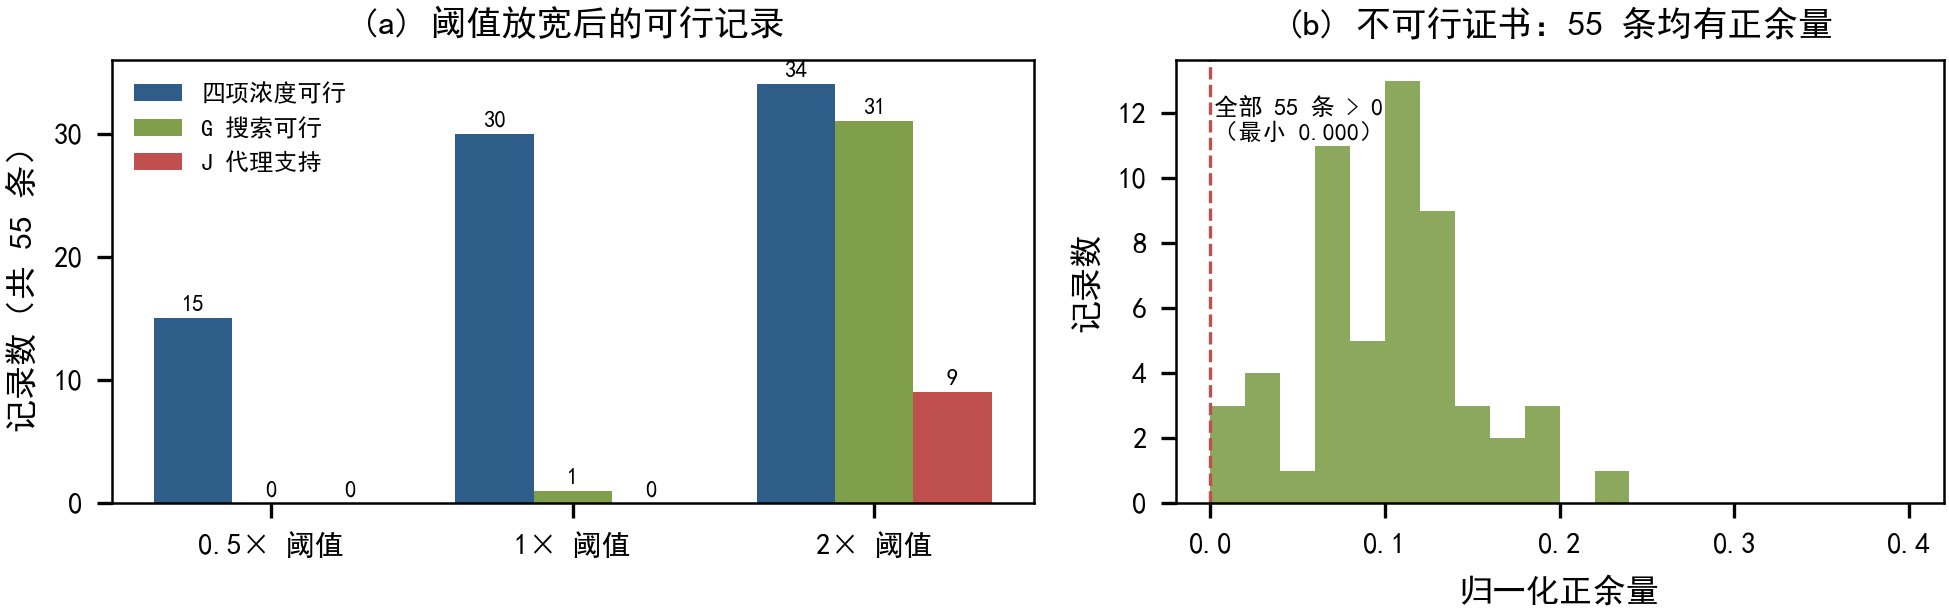
\includegraphics[width=0.98\textwidth]{figures/fig12_feasible.png}
\caption{(a) 缺陷阈值取 0.5 倍、1 倍、2 倍时，55 条记录中四项浓度可行、G 上搜索可行与 J 代理支持的条数；(b) 55 条不可行证书的归一化余量分布，全部大于 0。左图显示可行条数随阈值放宽而非线性增长，右图显示每条不可行记录都带正余量，即无解是结构性的而非求解失败。}
\label{fig:feas}
\end{figure*}

在化学可行的记录上叠加风格与 stale hops 约束，三层漏斗在 0.5 倍、1 倍、2 倍阈值下依次为：G 找到 0、1、31 条候选，J 复核后剩 0、0、9 条。阈值放宽到 2 倍时化学可行 34 条，其中 31 条能在 G 上找到风格候选，最终只剩 9 条通过 J，落差主要发生在代理层而不是化学层。联合复核把化学可行、风格可达与老化代理放在同一批记录上考察，任何一层不通过都不计为候选。2倍阈值下的9条是代理模型支持的重复划分记录，不是9款完成迁移的啤酒；其中3条来自T内部留出、对应3款来源酒。即便如此，最松的设置下 55 条记录也只产出 9 条通过两层代理的候选，不足六分之一，且都未经过真实品评。

阈值本身并不是常数。8.xlsx 的 261 行阈值只有 43 个给出数值，口径与基质（水、麦汁、成品酒）并不统一，文献值也依赖具体的品评方法。本文因此把阈值写成参数 $t_d$ 参与敏感性分析，而不是取固定数宣布可行。在这个设定下，第三问的答案是一个条件命题：逐项不增的严格协议下可行域为空且可被证书化；超额不增协议下部分记录的化学约束允许正份额；参考阈值下当前有限搜索没有候选通过联合代理复核；放宽阈值只能把这条窄缝拓宽，改变不了只有极少数配比能同时满足风格与缺陷的结构。

\section{模型评价与推广}\label{sec:eval}

\subsection{方法上的可取之处}

第一，评分端点不是"拍一个阈值"得到的。本文先从公开的 2197 条逐人评分重建面板均分与七级分布，再把连续与有序两类目标分开建模，使"预测均值"和"预测等级"各按自己的损失函数评价。第二，所有模型共享同一批按酒分层的划分，插补、截尾与标准化只在训练折内估计，因此不同方法之间的差值可比。第三，失败被完整保留：风格中位数基线几乎追平融合模型、图正则的收益随汇总口径变号、非零等级识别率只有约四分之一、严格浓度协议下55条记录的目标混配份额均为零——这些结果没有一项被删去或改写。

第四，本文把"无解"做成了可解释的结论。通过对偶可行性给出正余量证书，再逐项删除约束做消融，可以把笼统的"迁移不可行"定位到 DMS 与反式-2-壬烯醛这两个瓶颈上；同一套框架在参考阈值协议下得到30条四项化学约束允许正份额的记录；联合风格与stale hops代理检查后无候选通过。这比再多试几个生成模型更有信息量。

\subsection{局限}

\begin{enumerate}
\item[\textbf{L1}] \textbf{没有真实的感官验证。}全部结论建立在历史品评数据之上，生成谱与迁移候选的感官画像都是模型预测值。要证明一款候选酒真的好喝，需要新批次的化学测量与配对盲评，本文只给出了可执行的试验方案。
\item[\textbf{L2}] \textbf{品评人员在训练与测试之间重叠。}按酒划分能回答"新酒款"，不能回答"新面板"；16 名品评员的构成决定了结论的适用范围。人员留出设计尚未实现。
\item[\textbf{L3}] \textbf{缺失机制只做到压力测试。}MCAR、MAR、MNAR 与整块缺失四种机制给出了误差增量的量级，但没有建立与仪器检出限对应的缺失模型，因此 MNAR 的结果只能作为风险提示，不能外推为具体批次的偏差。
\item[\textbf{L4}] \textbf{化学侧未完成标定。}70 个可对照字段中 32 个存在 80 处不一致，检出限与回收率未知，5 个综合量的聚合公式未复原。第三问的浓度域分析因此限定在 61 个有单位记录的字段上。
\item[\textbf{L5}] \textbf{小样本生成难以全面胜出。}每种风格只有 3--31 款酒，约束凸组合提高了目标风格的识别率，却离真实分布更远；没有一种方法在保真度、覆盖度与复制率三个维度同时优于重采样。
\end{enumerate}

\subsection{可推广的部分}

代码层面，本文提供了两个可直接复用的入口：一是训练与无标签预测分离的流水线，输入只需与附件 1 一致的 231 列化合物字段，允许缺失、允许列序不同，输出面板均分、众数等级、中位数等级与七级概率四张表，并附带字段顺序、单位与输入哈希；二是"冻结候选—独立复核"的评测协议，可套用到任何"生成候选 + 模型打分"的任务上。

方法层面，本文的三点做法具有一般性。其一，当标签经过中心化/标准化而原始量表不可见时，先追查上游原始评分再重建端点，比在标准化刻度上强行反变换更可靠。其二，把"约束是否可行"表述为线性规划并给出不可行证书，可以在小样本条件下把失败转成工艺诊断。其三，对同一批留出预测同时报告单次拟合与重复聚合两种误差，可以避免"图模型有效/无效"这类依赖汇总口径的误判。

应用层面，该框架可迁移到其他发酵饮品（葡萄酒、清酒、酱油）的风味建模：只要具备"化合物谱 + 感官面板 + 风格标签"三要素，第一问的端点重建、第二问的模块级解释与第三问的可行域分析需要结合新任务的标定、评分和验证条件重新设计。

\section{结论}\label{sec:concl}

本文围绕啤酒风味的三项任务，先解决"评分端点从哪来"，再分别给出预测、解释与决策三类答案。

\textbf{第一问}：以 2197 条逐人 0--6 评分为依据重建了 50 个感官目标的面板均分与七级分布。按酒三折五次验证下，固定等权融合在核心 30 项上的均分误差为 0.50222 分，低于训练均值 0.60450 分，但只比风格中位数基线（0.50969 分）低 0.00747 分，差值的 95\% 重采样区间为 $[-0.01914,0.00418]$，含 0。该比较未提供融合模型稳定优于已知风格中位数基线的充分证据。新增同参数ET对照中，已知风格加化学比仅风格ET的核心MAE低0.01426分，表明在该模型设置下化学输入仍有预测信息；相对风格中位数的差值区间跨0。七级分布模型的累计分布平方距离为 0.02178（总体基线 0.02820），面板众数一致率 80.52\%，但非零众数一致率只有 24.33\%：总体一致率主要由 78.03\% 的零等级贡献，精细等级识别仍是短板。保形区间逐属性平均覆盖 90.06\%、平均宽 1.7342 分，但按品评人数分组后，3--4 人组只有 74.00\%。缺失机制实验进一步显示，系统性低值缺失（MNAR）使核心误差增加 0.0273 分，约为随机缺失 20\%（0.0139 分）的两倍。

\textbf{第二问}：231 个字段在 $|r|\ge0.7$ 下构成 109 条边的共表达图，但 150 个字段是孤立节点。图正则模型在单折口径下略差于无图（0.537035 对 0.536911）、在聚合口径下略好（0.524865 对 0.526148，区间 $[-0.002341,-0.000229]$），最终全数据模型选得 $\lambda=0$，即 Top-3 实际来自普通岭回归。150 条候选中有 36 条通过"频率 $\ge0.5$、至少 5 折入选、置换贡献为正"的描述性条件；把 80 个化学异常单元格置为缺失后 Top-3 保留 97.64\%，仅使用38个逐点一致字段、61个单位登记字段和226个非综合字段的32项交集时降至36.18\%，该交集与32个异常字段不重合。36条为满足描述性支持条件的候选，另外114条为探索性候选；网络用于描述共变结构，候选不代表因果效应。

\textbf{第三问}：三种风格各生成 40 条谱。受约束局部凸组合在 Tripel 上的平均目标风格概率为 0.3358、目标预测比例 0.695，均高于重采样的 0.2992 与 0.565，但分布距离 MMD$^2$ 反而更大（0.1158 对 0.1034），说明"更像目标风格"与"更接近真实分布"不是一回事。迁移任务中，55 条"来源 $\times$ 划分"记录上搜索可行 51 条、独立代理支持 11 条、再加原始尺度 stale hops 约束后 6 条；真实留出的 10 条记录（7 款酒）依次为 10、2、1 条。严格协议（四项浓度逐项不增）下最大 Tripel 份额全为 0，且 55 条记录都找到了正余量不可行证书，阻塞主要来自 DMS 与反式-2-壬烯醛；参考阈值下30条记录仅满足化学正份额条件，联合风格与stale hops检查后没有候选通过J代理复核；2倍阈值敏感性下有9条重复划分记录获得J代理支持，其中3条为T内部留出来源，均未经过新批次制备和盲评。

\textbf{总体判断}：在现有数据上，风格基线具有较强预测能力；化合物候选需要结合共变模块和单项稳定性解释；缺陷阈值、代理模型分歧与真实制备共同决定迁移结果。后续工作应按此顺序推进：先补人员留出与真实品评，再谈更复杂的模型。


\begin{thebibliography}{99}
\footnotesize

\bibitem{schreurs2024} Schreurs M, Piampongsant S, Roncoroni M, et al. Predicting and improving complex beer flavor through machine learning[J]. Nature Communications, 2024, 15: 2368. DOI: 10.1038/s41467-024-46346-0.

\bibitem{zenodo2026} Schreurs M, et al. Data from: Predicting and improving complex beer flavor through machine learning (Version v4)[DB/OL]. Zenodo, 2026. DOI: 10.5281/zenodo.23624915. 访问日期: 2026-10-25.

\bibitem{geurts2006} Geurts P, Ernst D, Wehenkel L. Extremely randomized trees[J]. Machine Learning, 2006, 63(1): 3--42.

\bibitem{friedman2001} Friedman J H. Greedy function approximation: a gradient boosting machine[J]. The Annals of Statistics, 2001, 29(5): 1189--1232.

\bibitem{breiman1996} Breiman L. Stacked regressions[J]. Machine Learning, 1996, 24(1): 49--64.

\bibitem{wolpert1992} Wolpert D H. Stacked generalization[J]. Neural Networks, 1992, 5(2): 241--259.

\bibitem{hastie2009} Hastie T, Tibshirani R, Friedman J. The Elements of Statistical Learning: Data Mining, Inference, and Prediction[M]. 2nd ed. New York: Springer, 2009: 219--243.

\bibitem{li2010} Li C, Li H. Variable selection and regression analysis for graph-structured covariates with an application to genomics[J]. The Annals of Applied Statistics, 2010, 4(3): 1498--1516.

\bibitem{lei2018} Lei J, G'Sell M, Rinaldo A, et al. Distribution-free predictive inference for regression[J]. Journal of the American Statistical Association, 2018, 113(523): 1094--1111.

\bibitem{gneiting2007} Gneiting T, Raftery A E. Strictly proper scoring rules, prediction, and estimation[J]. Journal of the American Statistical Association, 2007, 102(477): 359--378.

\bibitem{gretton2012} Gretton A, Borgwardt K M, Rasch M J, et al. A kernel two-sample test[J]. Journal of Machine Learning Research, 2012, 13: 723--773.

\bibitem{efron1993} Efron B, Tibshirani R J. An Introduction to the Bootstrap[M]. New York: Chapman \& Hall, 1993: 45--82.

\bibitem{vanbeneden2008} Vanbeneden N, Saison D, Delvaux F, et al. Decrease of 4-vinylguaiacol during beer aging and formation of apocynol and vanillin in beer[J]. Journal of Agricultural and Food Chemistry, 2008, 56(24): 11983--11988.

\bibitem{omur2012} Omur-Ozbek P, Dietrich A M, Duncan S E, et al. Role of lipid oxidation, chelating agents, and antioxidants in metallic flavor development in the oral cavity[J]. Journal of Agricultural and Food Chemistry, 2012, 60(9): 2274--2280.

\bibitem{pater2024} Pater A, Satora P, Januszek M. Effect of coriander seed addition at different stages of brewing on selected parameters of low-alcohol wheat beers[J]. Molecules, 2024, 29(4): 844.

\bibitem{meilgaard1993} Meilgaard M C. Individual differences in sensory threshold for aroma chemicals added to beer[J]. Food Quality and Preference, 1993, 4(3): 153--167.

\bibitem{santos2003} Santos J R, Carneiro J R, Guido L F, et al. Determination of E-2-nonenal by high-performance liquid chromatography with UV detection: assay for the evaluation of beer ageing[J]. Journal of Chromatography A, 2003, 985(1--2): 395--402.

\bibitem{lundberg2017} Lundberg S M, Lee S I. A unified approach to interpreting model predictions[C]//Advances in Neural Information Processing Systems 30. 2017: 4765--4774.

\end{thebibliography}

\vspace{1em}
\noindent\textbf{AI 工具使用声明}\quad 本文的数据核查、代码实现、图表绘制与文字整理使用了 OpenAI Codex 辅助；具体工具信息、使用时间、提示词、采纳内容与人工修改情况见支撑材料中的《AI 工具使用详情说明》。使用记录与队员独立复核情况以实际留存材料为准。


\appendix
\clearpage
\onecolumn
\section{全部 50 项的 Top-3 候选及证据分层}
\label{app:top3}

下表为全数据描述模型给出的最终 Top-3，括号内为固定全数据参数条件下200次bootstrap入选频率；标记 $^{\ast}$ 的36项同时满足频率、跨折入选和两类置换贡献条件，未标记的114项为探索性候选。标记根据未四舍五入的原始指标计算。最终模型选得 $\lambda=0$，即这些候选由普通岭回归系数给出；频率不是因果概率，也不是独立检验的 $p$ 值。

\begin{longtable}{L{0.30\columnwidth}L{0.62\columnwidth}}
\toprule
感官目标 & Top-3 字段（入选频率） \\
\midrule
\endfirsthead
\toprule
感官目标 & Top-3 字段（入选频率） \\
\midrule
\endhead
\bottomrule
\endfoot
A\_esters\_all & \texttt{acetaldehyde}$^{\ast}$（0.78）；\texttt{X.E..beta.ionone}（0.23）；\texttt{n.hexanol}（0.23） \\
A\_esters\_ethac & \texttt{acetaldehyde}（0.40）；\texttt{ethyl\_acetate}（0.21）；\texttt{cis.linalool.oxide}（0.17） \\
A\_esters\_flower & \texttt{beta.phellandrene}$^{\ast}$（0.56）；\texttt{X.E..alpha.ionone}（0.40）；\texttt{terpinolene}（0.14） \\
A\_esters\_fruity & \texttt{beta.phellandrene}$^{\ast}$（0.86）；\texttt{X1.10.di.epi.cubenol}（0.18）；\texttt{benzyl.alcohol}（0.30） \\
A\_esters\_isoaa & \texttt{n.hexanol}（0.40）；\texttt{ambroxide}（0.46）；\texttt{ethyl.hexadecanoate}（0.20） \\
A\_hops\_all & \texttt{iron}$^{\ast}$（0.56）；\texttt{DMS}（0.34）；\texttt{cis.dihydro.beta.terpineol}（0.20） \\
A\_hops\_citrus & \texttt{X6.methyl.5.hepten.2.one}$^{\ast}$（0.53）；\texttt{terpinolene}（0.19）；\texttt{geraniol}（0.26） \\
A\_hops\_noble & \texttt{iron}（0.36）；\texttt{ethyl\_octanoate}（0.23）；\texttt{ethyl\_decanoate}（0.16） \\
A\_hops\_tropical & \texttt{DMS}$^{\ast}$（0.55）；\texttt{beta.phellandrene}（0.26）；\texttt{citronellol}（0.29） \\
A\_hops\_woody & \texttt{iron}（0.27）；\texttt{ethyl\_2.methyl\_butyrate}（0.15）；\texttt{X2Z.6Z.farnesol}（0.23） \\
A\_malt\_all & \texttt{X2.acetylfuran}$^{\ast}$（0.77）；\texttt{ethyl.furoate}（0.42）；\texttt{phenethyl\_alcohol}（0.36） \\
A\_malt\_bread & \texttt{furfural}（0.36）；\texttt{ethyl.furoate}（0.28）；\texttt{ethyl.tiglate}（0.13） \\
A\_malt\_burn & \texttt{methylpyrazine}$^{\ast}$（0.75）；\texttt{X2.acetylfuran}$^{\ast}$（0.60）；\texttt{X4.methyl.1.pentanol}（0.11） \\
A\_malt\_cara & \texttt{X2.acetylfuran}$^{\ast}$（0.60）；\texttt{phenethyl\_alcohol}（0.45）；\texttt{octyl\_acetate}（0.31） \\
A\_malt\_grain & \texttt{gamma.nonalactone}（0.30）；\texttt{car.3.en.2.one}（0.36）；\texttt{X5.methylfurfural}（0.20） \\
F\_esters\_all & \texttt{acetaldehyde}$^{\ast}$（0.91）；\texttt{ethyl\_isovalerate}（0.34）；\texttt{n.hexanol}（0.27） \\
F\_esters\_ethac & \texttt{acetaldehyde}$^{\ast}$（0.51）；\texttt{ethyl\_acetate}（0.47）；\texttt{n.tetradecanol}（0.28） \\
F\_esters\_flower & \texttt{beta.phellandrene}（0.30）；\texttt{eucalyptol}（0.29）；\texttt{terpinolene}（0.13） \\
F\_esters\_fruity & \texttt{beta.phellandrene}（0.49）；\texttt{X.E..beta.ionone}（0.38）；\texttt{MeSH}（0.17） \\
F\_esters\_isoaa & \texttt{n.hexanol}（0.28）；\texttt{ethyl\_decanoate}（0.14）；\texttt{acetaldehyde}（0.12） \\
F\_hops\_all & \texttt{cis.dihydro.beta.terpineol}（0.70）；\texttt{iron}$^{\ast}$（0.70）；\texttt{ethyl\_isovalerate}（0.40） \\
F\_hops\_citrus & \texttt{geraniol}（0.47）；\texttt{citronellol}（0.43）；\texttt{cis.dihydro.beta.terpineol}（0.41） \\
F\_hops\_noble & \texttt{iron}$^{\ast}$（0.68）；\texttt{citronellol}（0.23）；\texttt{X14.hydroxy.alpha.humulene}（0.30） \\
F\_hops\_tropical & \texttt{X6.methyl.5.hepten.2.one}（0.46）；\texttt{DMS}（0.24）；\texttt{citronellol}（0.27） \\
F\_hops\_woody & \texttt{manool}（0.43）；\texttt{cis.dihydro.beta.terpineol}（0.28）；\texttt{n.octanol}（0.15） \\
F\_malt\_all & \texttt{acetaldehyde}$^{\ast}$（0.57）；\texttt{X2.acetylfuran}（0.47）；\texttt{X.E..alpha.ionone}（0.44） \\
F\_malt\_bread & \texttt{acetaldehyde}（0.26）；\texttt{dehydroxy.cis.linalool.oxide}（0.23）；\texttt{caryophylla.4.12..8.13..dien.5.alpha.ol}（0.15） \\
F\_malt\_burn & \texttt{X2.acetylfuran}$^{\ast}$（0.51）；\texttt{methylpyrazine}（0.57）；\texttt{MeSH}（0.25） \\
F\_malt\_cara & \texttt{acetaldehyde}（0.62）；\texttt{ethyl.nicotinate}（0.27）；\texttt{isobutyl.hexanoate}（0.23） \\
F\_malt\_grain & \texttt{X2.3.butanedione}（0.49）；\texttt{gamma.nonalactone}（0.14）；\texttt{X3.methyl.2.butenal}（0.18） \\
X4vg & \texttt{X4VG}$^{\ast}$（1.00）；\texttt{delta.terpinyl.acetate}（0.26）；\texttt{ethyl\_isovalerate}（0.22） \\
acetic & \texttt{lactic\_acid.mg.L.}（1.00）；\texttt{acetic\_acid.g.L.}（0.62）；\texttt{DES}（0.23） \\
acidity & \texttt{lactic\_acid.mg.L.}$^{\ast}$（1.00）；\texttt{acetic\_acid.g.L.}$^{\ast}$（0.72）；\texttt{X4.ethyl.guaiacol}（0.12） \\
aftertaste & \texttt{glycerol}$^{\ast}$（0.68）；\texttt{ethyl\_isovalerate}$^{\ast}$（0.62）；\texttt{cis.dihydro.beta.terpineol}（0.34） \\
alcohol & \texttt{acetaldehyde}$^{\ast}$（0.83）；\texttt{ethanol..v.v.}$^{\ast}$（0.82）；\texttt{X3.methyl.2.hexanol}（0.47） \\
barnyard & \texttt{X2.butyloctanoate}（0.32）；\texttt{gamma.eudesmol}（0.27）；\texttt{iron}（0.23） \\
bitternes & \texttt{iron}$^{\ast}$（0.98）；\texttt{cis.dihydro.beta.terpineol}（0.63）；\texttt{ethyl\_octanoate}（0.48） \\
body & \texttt{glycerol}$^{\ast}$（0.80）；\texttt{acetaldehyde}（0.68）；\texttt{X3.methyl.2.hexanol}（0.47） \\
clove & \texttt{linalool}$^{\ast}$（0.81）；\texttt{limonene}$^{\ast}$（0.67）；\texttt{eucalyptol}（0.48） \\
co2 & \texttt{ethyl\_octanoate}$^{\ast}$（0.62）；\texttt{X3.methyl.2.hexanol}（0.55）；\texttt{ethyl\_hexanoate}（0.34） \\
coriander & \texttt{x.methyl.1.octanol}$^{\ast}$（0.57）；\texttt{geraniol}$^{\ast}$（0.55）；\texttt{linalool}（0.46） \\
diacetyl & \texttt{CS2}（0.21）；\texttt{X.E..beta.ionone}（0.09）；\texttt{octyl\_acetate}（0.29） \\
dms & \texttt{SO2.mg.L.}$^{\ast}$（0.56）；\texttt{caryophylla.4.12..8.13..dien.5.alpha.ol}（0.18）；\texttt{neryl.formate}（0.17） \\
lactic & \texttt{lactic\_acid.mg.L.}（1.00）；\texttt{acetic\_acid.g.L.}（0.61）；\texttt{ethyl.phenylacetate}（0.28） \\
metallic & \texttt{iron}$^{\ast}$（0.94）；\texttt{ethyl\_isovalerate}（0.46）；\texttt{neryl.formate}（0.20） \\
orange & \texttt{X1.alpha.terpineol}$^{\ast}$（0.73）；\texttt{limonene}（0.49）；\texttt{linalool}（0.38） \\
overall & \texttt{ethyl\_acetate}（0.49）；\texttt{X2.butyloctanoate}（0.34）；\texttt{ethyl\_hexanoate}（0.14） \\
stale\_hops & \texttt{X2.butyloctanoate}（0.41）；\texttt{iron}（0.27）；\texttt{X.E..ortho.methoxy.cinnamaldehyde}（0.21） \\
sweetness & \texttt{ethyl\_decanoate}$^{\ast}$（0.81）；\texttt{iron}$^{\ast}$（0.52）；\texttt{ethyl\_octanoate}（0.28） \\
t2n & \texttt{germacrene.D}$^{\ast}$（0.58）；\texttt{isopentyl.hexanoate}（0.46）；\texttt{X.Z..dihydro.apofarnesal}（0.18） \\
\end{longtable}

150 条记录中，满足“入选频率 $\ge0.5$、至少 5 个训练折入选、普通与风格内置换贡献均为正”这三条描述性条件的有 36 条。完整记录（含系数方向、置换贡献、单位与文献核查状态）见支撑材料 \texttt{top3\_with\_evidence.csv}。
\section{敏感性分析所用32字段清单}\label{app:fieldsets}
该集合为全部可比记录尺度一致、在浓度单位注册表中、且属于226个非综合输入的字段交集；与含80处不一致的32个字段没有重合。单位为来源表的参考单位；部分建模输入仍为对数变换值，\texttt{diethyl.succinate} 为恒等对应，单位登记本身不证明化学定值准确。
\begin{longtable}{L{0.37\columnwidth}L{0.10\columnwidth}L{0.37\columnwidth}L{0.10\columnwidth}}
\toprule
字段 & 单位 & 字段 & 单位\\
\midrule
\endfirsthead
\toprule
字段 & 单位 & 字段 & 单位\\
\midrule
\endhead
\bottomrule
\endfoot
\texttt{acetaldehyde} & mg/L & \texttt{MeSH} & $\mu$g/L \\
\texttt{CS2} & $\mu$g/L & \texttt{octyl\_acetate} & mg/L \\
\texttt{DES} & $\mu$g/L & \texttt{phenethyl\_acetate} & mg/L \\
\texttt{DMS} & $\mu$g/L & \texttt{phenethyl\_alcohol} & mg/L \\
\texttt{ethyl\_2.\allowbreak{}methyl\_butyrate} & mg/L & \texttt{X4VG} & mg/L \\
\texttt{ethyl\_acetate} & mg/L & \texttt{SO2.\allowbreak{}mg.\allowbreak{}L.\allowbreak{}} & mg/L \\
\texttt{ethyl\_decanoate} & mg/L & \texttt{acetic\_acid.\allowbreak{}g.\allowbreak{}L.\allowbreak{}} & g/L \\
\texttt{ethyl\_hexanoate} & mg/L & \texttt{ammonia.\allowbreak{}mg.\allowbreak{}L.\allowbreak{}} & mg/L \\
\texttt{ethyl\_isovalerate} & mg/L & \texttt{betaglucan.\allowbreak{}mg.\allowbreak{}L.\allowbreak{}} & mg/L \\
\texttt{ethyl\_octanoate} & mg/L & \texttt{lactic\_acid.\allowbreak{}mg.\allowbreak{}L.\allowbreak{}} & mg/L \\
\texttt{ethyl\_propionate} & mg/L & \texttt{glycerol} & g/L \\
\texttt{H2S} & $\mu$g/L & \texttt{iron} & mg/L \\
\texttt{isoamyl\_alcohol} & mg/L & \texttt{protein.\allowbreak{}g.\allowbreak{}L.\allowbreak{}} & g/L \\
\texttt{isobutanol} & mg/L & \texttt{GFS} & g/L \\
\texttt{isobutyl\_acetate} & mg/L & \texttt{ethanol.\allowbreak{}.\allowbreak{}v.\allowbreak{}v.\allowbreak{}} & v/v \\
\texttt{isopentyl\_acetate} & mg/L & \texttt{diethyl.\allowbreak{}succinate} & mg/L \\
\end{longtable}

\section{源程序清单}
\label{app:code}

全部源程序随支撑材料提交，运行环境为 Python 3.12、依赖版本见 \texttt{requirements-lock.txt}。下表给出模块与章节的对应关系；此后的完整清单按 \texttt{src/}、\texttt{scripts/}、\texttt{tests/}、入口脚本与配置文件顺序排列。

\begin{table}[h]
\centering\footnotesize\renewcommand{\arraystretch}{1.1}
\caption{核心模块与对应章节}
\begin{tabular}{L{0.42\columnwidth}L{0.30\columnwidth}L{0.18\columnwidth}}
\toprule
文件 & 功能 & 章节 \\
\midrule
src/audit.py & 附件结构、字段尺度、模板公式核查 & 3 \\
src/data.py & 数据读入、按酒对齐、缺失与截尾 & 3--4 \\
src/common.py & 划分、预处理管线、随机种子 & 4--6 \\
src/q1.py & 面板均分与七级分布的基线模型 & 4 \\
src/q2.py & 共表达图构建与岭回归候选 & 5 \\
src/q3.py & 风格生成与迁移搜索原型 & 6 \\
src/stage2.py & 保形区间、分级敏感性、置换贡献 & 4--5 \\
src/stage3\_algorithms.py & 图正则求解、对偶证书、阈值风险函数 & 5--6 \\
src/stage3\_generation.py & 四种生成器与 MMD/KS/复制率评价 & 6 \\
src/stage3\_graph.py & 交叉拟合的图消融与因素稳定性 & 5 \\
src/stage3\_prediction.py & 嵌套预测与保形区间 & 4 \\
src/stage4\_audit.py & 原始评分重建、化学尺度与 OAV 复核 & 3 \\
src/stage4\_models.py & 有序分布模型与评分规则 & 4 \\
src/deployment.py & 无标签预测入口与输入校验 & 7 \\
run.py / run\_stage2.py / run\_stage3.py / run\_stage4.py & 四个阶段的命令行入口 & 全文 \\
run\_final\_model.py & 最终模型训练与预测 & 7 \\
\bottomrule
\end{tabular}
\end{table}

\begingroup\scriptsize
以下列出建模、审计、实验与验证程序。论文排版与图形生成脚本（\texttt{prepare\_*.py}、\texttt{build\_*.py}、\texttt{render\_*.py}、\texttt{verify\_*.py} 等）不属于建模程序，随支撑材料提交，此处不重复列出。
\subsection*{\texttt{001\_\_\_init\_\_.py}}
\lstinputlisting{sources/001___init__.py}
\subsection*{\texttt{002\_audit.py}}
\lstinputlisting{sources/002_audit.py}
\subsection*{\texttt{003\_common.py}}
\lstinputlisting{sources/003_common.py}
\subsection*{\texttt{004\_data.py}}
\lstinputlisting{sources/004_data.py}
\subsection*{\texttt{005\_q1.py}}
\lstinputlisting{sources/005_q1.py}
\subsection*{\texttt{006\_q2.py}}
\lstinputlisting{sources/006_q2.py}
\subsection*{\texttt{007\_q3.py}}
\lstinputlisting{sources/007_q3.py}
\subsection*{\texttt{008\_reporting.py}}
\lstinputlisting{sources/008_reporting.py}
\subsection*{\texttt{009\_stage2.py}}
\lstinputlisting{sources/009_stage2.py}
\subsection*{\texttt{010\_stage3\_algorithms.py}}
\lstinputlisting{sources/010_stage3_algorithms.py}
\subsection*{\texttt{011\_stage3\_generation.py}}
\lstinputlisting{sources/011_stage3_generation.py}
\subsection*{\texttt{012\_stage3\_graph.py}}
\lstinputlisting{sources/012_stage3_graph.py}
\subsection*{\texttt{013\_stage3\_prediction.py}}
\lstinputlisting{sources/013_stage3_prediction.py}
\subsection*{\texttt{014\_stage4\_audit.py}}
\lstinputlisting{sources/014_stage4_audit.py}
\subsection*{\texttt{015\_stage4\_models.py}}
\lstinputlisting{sources/015_stage4_models.py}
\subsection*{\texttt{016\_stage4\_trial.py}}
\lstinputlisting{sources/016_stage4_trial.py}
\subsection*{\texttt{017\_analyze\_trial.py}}
\lstinputlisting{sources/017_analyze_trial.py}
\subsection*{\texttt{020\_fetch\_stage4\_sources.py}}
\lstinputlisting{sources/020_fetch_stage4_sources.py}
\subsection*{\texttt{030\_stage3\_preflight.py}}
\lstinputlisting{sources/030_stage3_preflight.py}
\subsection*{\texttt{032\_stage4\_graph\_comparison.py}}
\lstinputlisting{sources/032_stage4_graph_comparison.py}
\subsection*{\texttt{036\_verify\_stage3.py}}
\lstinputlisting{sources/036_verify_stage3.py}
\subsection*{\texttt{037\_verify\_stage4.py}}
\lstinputlisting{sources/037_verify_stage4.py}
\subsection*{\texttt{038\_test\_invariants.py}}
\lstinputlisting{sources/038_test_invariants.py}
\subsection*{\texttt{039\_test\_stage2.py}}
\lstinputlisting{sources/039_test_stage2.py}
\subsection*{\texttt{040\_test\_stage3\_algorithms.py}}
\lstinputlisting{sources/040_test_stage3_algorithms.py}
\subsection*{\texttt{041\_test\_stage3\_research.py}}
\lstinputlisting{sources/041_test_stage3_research.py}
\subsection*{\texttt{042\_test\_stage4.py}}
\lstinputlisting{sources/042_test_stage4.py}
\subsection*{\texttt{043\_run.py}}
\lstinputlisting{sources/043_run.py}
\subsection*{\texttt{044\_run\_stage2.py}}
\lstinputlisting{sources/044_run_stage2.py}
\subsection*{\texttt{045\_run\_stage3.py}}
\lstinputlisting{sources/045_run_stage3.py}
\subsection*{\texttt{046\_run\_stage4.py}}
\lstinputlisting{sources/046_run_stage4.py}
\subsection*{\texttt{047\_config.json}}
\lstinputlisting{sources/047_config.json}
\subsection*{\texttt{048\_config\_stage2.json}}
\lstinputlisting{sources/048_config_stage2.json}
\subsection*{\texttt{049\_config\_stage3.json}}
\lstinputlisting{sources/049_config_stage3.json}
\subsection*{\texttt{050\_config\_stage3\_design.json}}
\lstinputlisting{sources/050_config_stage3_design.json}
\subsection*{\texttt{051\_config\_stage4.json}}
\lstinputlisting{sources/051_config_stage4.json}
\subsection*{\texttt{052\_review\_experiments.py}}
\lstinputlisting{sources/052_review_experiments.py}
\subsection*{\texttt{053\_review\_diagnostics.py}}
\lstinputlisting{sources/053_review_diagnostics.py}
\subsection*{\texttt{055\_run\_final\_model.py}}
\lstinputlisting{sources/055_run_final_model.py}
\subsection*{\texttt{056\_deployment.py}}
\lstinputlisting{sources/056_deployment.py}
\subsection*{\texttt{057\_diagnose\_stage4.py}}
\lstinputlisting{sources/057_diagnose_stage4.py}
\subsection*{\texttt{058\_test\_deployment.py}}
\lstinputlisting{sources/058_test_deployment.py}
\subsection*{\texttt{059\_ordinal\_two\_stage\_experiment.py}}
\lstinputlisting{sources/059_ordinal_two_stage_experiment.py}
\subsection*{\texttt{060\_summarize\_two\_stage.py}}
\lstinputlisting{sources/060_summarize_two_stage.py}
\subsection*{\texttt{061\_joint\_review\_experiments.py}}
\lstinputlisting{sources/061_joint_review_experiments.py}
\subsection*{\texttt{062\_test\_joint\_review.py}}
\lstinputlisting{sources/062_test_joint_review.py}
\endgroup
\subsection*{补充核查程序}
\lstinputlisting{sources/063_submission_review_checks.py}
\lstinputlisting{sources/064_submission_graph_grid.py}
\lstinputlisting{sources/065_submission_scale_figure.py}

\lstinputlisting{sources/066_submission_style_increment.py}


\end{document}

